\documentclass[english,letter paper,12pt,reqno]{article}
\usepackage{etex} % to fix "no room for new dimen" error. Voodoo.
\usepackage{array}
\usepackage{bussproofs}
\usepackage{stmaryrd}
\usepackage{amsmath, amscd, amssymb, mathrsfs, accents, amsfonts,amsthm}
\usepackage[all]{xy}
\usepackage{mathtools} % for bra-ket
\usepackage{tikz}
\usetikzlibrary{calc}

\AtEndDocument{\bigskip{\footnotesize%
  \textsc{Department of Mathematics, University of Southern California} \par  
  \textit{E-mail address}: \texttt{murfet@usc.edu} \par
}}

% Labels in tabular
\newcommand{\tagarray}{\mbox{}\refstepcounter{equation}$(\theequation)$}

% Bra-ket stuff
\DeclarePairedDelimiter\bra{\langle}{\rvert}
\DeclarePairedDelimiter\ket{\lvert}{\rangle}
\DeclarePairedDelimiterX\braket[2]{\langle}{\rangle}{#1 \delimsize\vert #2}
\DeclarePairedDelimiterX\inner[2]{\langle}{\rangle}{#1,#2}
\DeclarePairedDelimiter\abs{\lvert}{\rvert}
\DeclarePairedDelimiter\norm{\lVert}{\rVert}
\DeclarePairedDelimiter\set{\lbrace}{\rbrace}

%\begin{align*}
%\bra{a}       &= \bra*{\frac{a}{1}}\    \ket{a}       &= \ket*{\frac{a}{1}}\    \braket{a}{b} &= \braket*{\frac{a}{1}}{\frac{b}{1}}\    %\inner{a}{b}  &= \inner*{\frac{a}{1}}{\frac{b}{1}}\    \abs{a}       &= \abs*{\frac{a}{1}}\    \norm{a}      &= \norm*{\frac{a}%{1}}\    \set{a,b}     &= \set*{\frac{a}{1},\frac{b}{1}}
%\end{align*}

% TikZ stuff
\def\drawbang{\draw[color=teal!50, line width=2pt]}
\def\drawprom{\draw[color=gray, line width=3pt]}
\def\bluenode{\node[circle,draw=blue!50,fill=blue!20]}
\def\mapnode{\node[circle,draw=black,fill=black,inner sep=0.5mm]}
\def\whitenode{\node[circle,draw=blue!50,fill=blue!5]}
\def\dernode{\node[circle,draw=black,fill=white]}
\definecolor{Myblue}{rgb}{0,0,0.6}
\usepackage[a4paper,colorlinks,citecolor=Myblue,linkcolor=Myblue,urlcolor=Myblue,pdfpagemode=None]{hyperref}

\SelectTips{cm}{}

\setlength{\evensidemargin}{0.1in}
\setlength{\oddsidemargin}{0.1in}
\setlength{\textwidth}{6.3in}
\setlength{\topmargin}{0.0in}
\setlength{\textheight}{8.5in}
\setlength{\headheight}{0in}

\newtheorem{theorem}{Theorem}[section]
\newtheorem{proposition}[theorem]{Proposition}
\newtheorem{lemma}[theorem]{Lemma}
\newtheorem{corollary}[theorem]{Corollary}

\newtheoremstyle{example}{\topsep}{\topsep}
	{}
	{}
	{\bfseries}
	{.}
	{2pt}
	{\thmname{#1}\thmnumber{ #2}\thmnote{ #3}}
	
	\theoremstyle{example}
	\newtheorem{definition}[theorem]{Definition}
	\newtheorem{example}[theorem]{Example}
	\newtheorem{remark}[theorem]{Remark}
	\newtheorem{question}[theorem]{Question}

\numberwithin{equation}{section}

% Operators
\def\eval{\operatorname{ev}}
\def\sh{\operatorname{Sh}}
\def\res{\operatorname{Res}}
\def\Coker{\operatorname{Coker}}
\def\Ker{\operatorname{Ker}}
\def\im{\operatorname{Im}}
\def\can{\operatorname{can}}
\def\K{\mathbf{K}}
\def\D{\mathbf{D}}
\def\N{\mathbf{N}}
\def\LG{\mathcal{LG}}
\def\Ab{\operatorname{Ab}}
\def\Hom{\operatorname{Hom}}
\def\modd{\operatorname{mod}}
\def\Modd{\operatorname{Mod}}
\DeclareMathOperator{\Ext}{Ext}
\DeclareMathOperator{\Tr}{Tr}
\DeclareMathOperator{\End}{End}
\DeclareMathOperator{\rank}{rank}
\DeclareMathOperator{\tot}{Tot}
\DeclareMathOperator{\ch}{ch}
\DeclareMathOperator{\str}{str}
\DeclareMathOperator{\hmf}{hmf}
\DeclareMathOperator{\HMF}{HMF}
\DeclareMathOperator{\hf}{HF}
\DeclareMathOperator{\At}{At}
\DeclareMathOperator{\Cat}{Cat}
\DeclareMathOperator{\Spec}{Spec}
\DeclareMathOperator{\MSpec}{MSpec}
\DeclareMathOperator{\Sym}{Sym}
\DeclareMathOperator{\LC}{LC}
\def\inta{\bold{int}}
\def\contract{\;\lrcorner\;}

% SCprooftree environment
\newenvironment{scprooftree}[1]
{\gdef\scalefactor{#1}\begin{center}\proofSkipAmount \leavevmode}
{\scalebox{\scalefactor}{\DisplayProof}\proofSkipAmount \end{center} }
  
\begin{document}

% Bussproof things
\def\ScoreOverhang{1pt}

% Commands
\def\Res{\res\!}
\newcommand{\ud}[1]{\operatorname{d}\!{#1}}
\newcommand{\Ress}[1]{\res_{#1}\!}
\newcommand{\cat}[1]{\mathcal{#1}}
\newcommand{\lto}{\longrightarrow}
\newcommand{\xlto}[1]{\stackrel{#1}\lto}
\newcommand{\mf}[1]{\mathfrak{#1}}
\newcommand{\md}[1]{\mathscr{#1}}
\newcommand{\church}[1]{\underline{#1}}
\newcommand{\prf}[1]{\underline{#1}}
\newcommand{\den}[1]{\llbracket #1 \rrbracket}
\def\l{\,|\,}
\def\sgn{\textup{sgn}}
\def\cont{\operatorname{cont}}

\title{Logic and linear algebra: an introduction}
\author{Daniel Murfet}

\maketitle

\begin{abstract} We give an introduction to computation and logic tailored for algebraists, with a focus on explaining how to represent programs in the $\lambda$-calculus and proofs in linear logic as linear maps between vector spaces. The interesting part of this vector space semantics is based on the cofree cocommutative coalgebra of Sweedler \cite{sweedler} and the recent explicit computations of liftings in \cite{murfet_coalg}.
\end{abstract}

\section{Introduction}

The purpose of this note is to use linear algebra to give an introduction to logic, specifically Girard's linear logic \cite{girard_llogic}. In mathematical logic the objects of study are \emph{proofs}, just as manifolds, knots or representations are the objects in other disciplines of mathematics. The reader will no doubt agree that proofs  can be complicated, and it is therefore not surprising that there are multiple ways of approaching their study. The most popular styles of formalising mathematical proofs are Hilbert style systems, which most mathematicians will be exposed to as undergraduates, and natural deduction or sequent calculus systems. What these systems share is that they are about propositions and their proofs, which are constructed from axioms via a series of deduction rules. However the set of axioms and deduction rules, and the way of formatting proofs, varies from system to system. 

Following Frege and Gentzen, natural deduction and sequent calculus systems format their proofs using a $2$-dimensional notation where the flow of logical argument proceeds from top to bottom and hypotheses are arranged from left to right. For example, here is a proof formalised in the sequent calculus of linear logic:
\begin{center}
\AxiomC{}
\UnaryInfC{$A \vdash A$}
\AxiomC{}
\UnaryInfC{$A \vdash A$}
\AxiomC{}
\UnaryInfC{$A \vdash A$}
\RightLabel{\scriptsize$\multimap L$}
\BinaryInfC{$A, A \multimap A \vdash A$}
\RightLabel{\scriptsize$\multimap L$}
\BinaryInfC{$A, A \multimap A, A \multimap A \vdash A$}
\RightLabel{\scriptsize$\multimap R$}
\UnaryInfC{$A \multimap A, A \multimap A \vdash A \multimap A$}
\alwaysDoubleLine
\RightLabel{\scriptsize der}
\UnaryInfC{$!( A \multimap A ), !(A \multimap A) \vdash A \multimap A$}
\alwaysSingleLine
\RightLabel{\scriptsize ctr}
\UnaryInfC{$!( A \multimap A) \vdash A \multimap A$}
\DisplayProof
\qquad
\tagarray{\label{church_2_intro}}
\end{center}
Here the proposition that is being proved is the final line, the sequent ${!} (A \multimap A ) \vdash A \multimap A$. To fully explain the content of this proof we would need to introduce the connectives ${!}, \multimap$ of linear logic and the deduction rules that are used to pass from one row to the next. All of this we will do in Section \ref{??}, but we can more directly provide some intuition by employing the \emph{semantics} of linear logic, by which we mean a faithful representation of the internal structure of the logic in another mathematical structure. In this note, the relevant mathematical structures are vector spaces and linear maps. In the semantics we will define $A$ will be represented by a vector space $V$, $A \multimap A$ by the space of endomorphisms of $V$, and $!(A \multimap A)$ by the cofree coalgebra generated by this space of endomorphisms. The representation of the proof given above is simply a function which \emph{takes an endomorphism of $V$ and squares it}. 

%Without trying to explain all the details, let us briefly describe what this proof is about. At the top are axioms $A \vdash A$ which may be read as ``$A$ implies $A$''. Deduction rules are indicated by horizontal lines and proceed from their hypotheses (in the numerator) to their conclusion (in the denominator). They are labelled by the names $\multimap L, \multimap R, \ldots$ of the deduction rule which is being used. The argument continues downards until we reach the desired sequent ${!} (A \multimap A) \vdash A \multimap A$.

With this preparation, the reader will not be surprised to learn that for each integer $n$ there is a proof in linear logic of the sequent ${!} (A \multimap A ) \vdash A \multimap A$ which is represented in the semantics by taking an endomorphism and raising it to the $n$th power. And it is not only natural numbers that can be encoded this way as proofs: one can encode computable \emph{functions} $\mathbb{N} \lto \mathbb{N}$ and a wide range of other programs. In this way we see that the \emph{set} of possible proofs of a sequent carries a rich and interesting structure. From one point of view it is these structured sets that are the subject of proof theory and related areas of computer science. %This can be seen as an example of the Curry-Howard correspondence, which matches proofs in certain logics with programs in programming languages like the $\lambda$-calculus.This perspective, which emphasises the structure of the \emph{set} of possible proofs, is emblematic of the age of computation: 

\vspace{0.5cm}

There are many excellent and comprehensive introductions to linear logic \cite{girard_llogic, mellies, abramsky}. Our aim is rather to give an opinionated view highlighting those aspects that we think are of particular interest for algebraists. Linear logic is relevant to algebra because shadows of proofs in linear logic arise naturally in algebraic contexts whenever there is an interaction between \emph{linear} objects (e.g. vector bundles) and the \emph{non-linear} objects which classify them (e.g. moduli spaces of vector bundles). We have in mind the following kind of situation: let $\cat{B}$ be a bicategory which we think of as having algebraic spaces as objects and some kind of correspondences or integral transforms as $1$-morphisms. Two of the assumptions we make about this bicategory are:
\begin{itemize}
\item[(i)] It is symmetric monoidal and closed, so that for a pair of objects $v,w$ we may form $v \otimes w$ and $\Hom(v,w)$, and
\item[(ii)] for each pair of objects $v,w$ there is a reasonable moduli space $\mathscr{M}_{v,w}$ whose points are in bijection with $1$-morphisms $v \lto w$ in $\cat{B}$ and that these moduli spaces themselves form valid objects of $\cat{B}$.
\end{itemize}
It therefore makes sense to ask for a ``universal'' $1$-morphism $\mathscr{M}_{v,w} \lto \Hom(v,w)$ whose value over a point $[X]$ of the moduli space corresponding to $X: v \lto w$ is $X$ itself.

In this situation we can expect to find a semantics of linear logic in the bicategory $\cat{B}$. For instance, if the formula $A$ of the logic is assigned the object $v$ of the bicategory, then the proof \eqref{church_2_intro} given above is represented by a $1$-morphism
\[
\mathscr{M}_{v,v} \lto \Hom(v,v)
\]
whose value over a point $[X]$ of $\mathscr{M}_{v,v}$ is the square $X \circ X$ of a loop $X: v \lto v$. In this way arbitrary integers, encoded as proofs in linear logic, may be represented as $1$-morphisms in $\cat{B}$, and the same is true any program computing integers from integers that can be encoded in linear logic. The remarkable thing is that all of this structure is immediately present as soon as we allow the objects $\Hom(v,w)$ to interact with their own moduli spaces. In \cite{??} and its forthcoming sequels this is made precise when $\cat{B}$ is a bicategory of matrix factorisations.

% but it may come as a surprise that some of the techniques invented by logicians to study proofs are closely related to constructions in modern algebra and category theory, such as symmetric monoidal categories and functors between them. 

%For example, in \emph{linear logic}  any proof of a formula can be viewed as a decorated graph called a proof-net which is similar in some ways to a bordism or a string diagram, and the semantics of linear logic \cite{mellies} can be intuitively understood in terms of functors from a symmetric monoidal category of formulas (the objects) and proofs (the morphisms) to other monoidal categories, including the category of vector spaces.\footnote{Unfortunately there does not yet appear to be a formal statement in the literature to the effect that the set of categorical semantics of linear logic is in bijection with functors out of some free category generated by the syntax, but nonetheless we feel this is a helpful motivating perspective.}

%This invites a comparison to the subject of topological field theory \cite{atiyah,witten} which may be described as the study of monoidal functors from categories of bordisms to the category of vector spaces. However, there is a crucial difference which makes the semantics of linear logic more interesting in some ways than representations of a category of bordisms: proofs are \emph{nonlinear} objects, and their semantics is therefore highly infinite. To illustrate how this nonlinearity manifests itself in algebraic semantics, suppose we are given rings $A,B$ and a $B$-$A$-bimodule $X$. A basic operation is the linear functor
%\begin{equation}
%M \longmapsto X \otimes_A M
%\end{equation}
%from the category of left $A$-modules to the category of left $B$-modules. By analogy with the language of analysis, $X$ is sometimes referred to as a ``kernel''. This kind of operation on modules is fundamental in the algebra of higher-dimensional topological field theory where defects between field theories are represented by bimodules of various kinds \cite{??}.

%An operation that does not arise as naturally in that context is the following ``quadratic'' map defined on $A$-$A$-bimodules $X$ (that is, in the situation where $A = B$)
%\begin{equation}\label{eq:church_as_bimod}
%X \longmapsto X \otimes_A X\,.
%\end{equation}
%This operation is nonlinear and cannot be represented by tensoring with some bimodule. Nonetheless there \emph{is} a good notion of such nonlinear kernels: they are called \emph{programs}, and the operation above is an incarnation of the Church numeral $\church{2}$ in the $\lambda$-calculus. In this note we will discuss Church numerals and their semantics in the simple setting of vector spaces. Making the above comments about bimodules and programs precise requires the construction of \emph{bicategorical} semantics of linear logic, where the ``squaring program'' $\church{2}$ of \eqref{eq:church_as_bimod} can be interpreted as a kind of bundle over the space parametrising suitable bimodules $X$, whose fibre over a point $[X]$ is the square $X \otimes_A X$. This idea will be made precise in \cite{??,??} using matrix factorisations (which are bimodules equipped with an additional operator) and a bicategory which extends the bicategory of Landau-Ginzburg models studied in the context of topological field theory \cite{??}. 

% We take the point of view that semantics of linear logic ``lurks'' just beyond the boundaries of subjects of topological field theory, and interaction between the two subjects is likely to be rewarding for both.

% These parametrising spaces are the ``infinite'' content reflecting the non-linearity, but they are finite in the context of algebraic geometry where they are cut out of affine spaces $\mathbb{C}^n$ by finite numbers of polynomial equations.

% Such novel semantics defined using algebra might be of interest of a proof theorist, but what is there in logic for the algebraist? The author cannot presume to speak for experts in logic, but he can explain the source of his own fascination with the subject. After the work of Turing, G\"odel and Church \cite{soare} computation has become a fundamental concept in mathematics, and we have a good understanding of which functions are computable. But what kind of thing is the \emph{process} of computation? One answer is that computation is what happens when a Turing machine is iterated, during the $\beta$-reduction process of the $\lambda$-calculus, or during the cut-elimination process of logic. These models of computation are equivalent, but each is tied to specific syntax. What is the common essence of these processes? This is a question as deep as ``What is space?'' and it would be absurd to expect conclusive answers \cite{denning}. Nonetheless such questions generate interesting mathematics, a recent example being homotopy type theory \cite{univalent,warren}, and the tools developed in the last few decades of research into higher categories, topological field theory and algebraic geometry offer many interesting avenues of concrete investigation.

\vspace{0.5cm}

Most of what we have to say is well-known, with the exception of some aspects of the vector space semantics in Section \ref{section:vector_space_sem}. There are many aspects of logic and its connections with other subjects that we cannot cover: for a well-written account of analogies between logic, topology and physics we recommend the survey of Baez and Stay \cite{baez}.
\\

The first aspect of logic that we choose for special emphasis is the already mentioned \emph{nonlinearity} represented in linear logic by the exponential modality, which corresponds in the vector space semantics to forming from a vector space $V$ the universal cocommutative coalgebra ${!}V$ whose coproduct is the universal way of duplicating elements of $V$. Through an embedding of a prototypical programming language called the $\lambda$-calculus into linear logic we will see how the exponential modality is the aspect of logic responsible for the capability of programs to use their inputs more than once.

% This reuse -- which is demonstrated in the ``program'' \eqref{eq:church_as_bimod} which uses the input bimodule $M$ twice -- is a form of non-linearity, which is moreover the source of all the interesting complexity of non-trivial programs.\footnote{It might seem odd that the first aspect of linear logic that we choose to emphasise is non-linearity. But the point of linear logic is not that everything is linear. Classical logic is a mix of linear and non-linear components, and the insight of Girard with linear logic is that it is possible to create a refinement where there is an explicit boundary between these two worlds, and there are special language features -- such as the exponential modality -- to manage transitions across this boundary.}

The second particularly interesting aspect of logic is \emph{cut-elimination}. This is a fundamental feature of logic going back to Gentzen \cite{gentzen} which may be described (superficially) as the answer to the following question: given two composable functions $f,g$ given by algorithms, what is the simplest form of the algorithm computing $g \circ f$? LINK BACK to earlier comments about what is computation This is linked to deep questions about the nature of computation, as elucidated by Girard \cite{girard_towards}.
\\
%Here is how we imagine potential readers of this article: either a computer scientist or logician interested in the semantics of the exponential modality in linear logic and connections between proof theory and geometry, or an algebraist or mathematical physicist who likes symmetric monoidal categories and is curious about the boundary between the finite (in the sense of dualisability of objects in topological field theory) and the infinite (in the sense of infinite coproducts) and who might appreciate learning that logicians have their own way of probing the realm between finite and infinite, with deep roots. 

The outline of the article is as follows: in Section \ref{section:logic} we introduce the $\lambda$-calculus, intuitionistic logic and linear logic, with an emphasis on the role of duplication. In Section \ref{section:diagrammatics} we assign to every proof in intuitionistic linear logic a string diagram and corresponding linear map, and give a detailed example. In Section \ref{section:cut_elim} we turn to cut-elimination, examining a mildly non-trivial example in detail. In Appendix \ref{section:example_lifting} we examine tangent maps in connection with proofs in linear logic. 
\\

\emph{Acknowledgements.} Thanks to Nils Carqueville, Jesse Burke, and Andante.
\\

Throughout $k$ is an algebraically closed field of characteristic zero.

\section{Logic}\label{section:logic}

We begin with a brief introduction to the $\lambda$-calculus (Section \ref{section:lambda_calc}) and introduce our basic example, the Church numeral $\church{2}$. Then we move on to discuss intuitionistic logic (Section \ref{section:intuit_logic}) and the Curry-Howard correspondence which shows that the simply-typed $\lambda$-calculus is isomorphic to intuitionistic logic, under the slogan ``proofs are programs''. As foreshadowed in the introduction, we pay particular attention to the role of nonlinearity of proofs and programs, which manifests itself in the role of duplication of terms in the $\lambda$-calculus and the contraction rule in logic. This nonlinearity, implicit in classical logic, is made explicit in a refinement of classical logic due to Girard, called Linear Logic (Section \ref{section:intro_ll}). For more details see \cite{girard_prooftypes,mellies} or, for the reader with a lunch break to spare \cite{scott_talk}.

\subsection{The $\lambda$-calculus}\label{section:lambda_calc}

At the same time as Turing defined his machines, Church gave another formalisation of the intuitive idea of a computable function in terms of what he called the $\lambda$-calculus \cite{church,selinger}. Both concepts identify the same class of computable functions $\mathbb{N} \lto \mathbb{N}$, but the $\lambda$-calculus is much more natural from the point of category theory, and it also serves as the theoretical underpinning of programming languages like Lisp \cite{mccarthy}. Intuitively, while Turing machines make precise the concept of \emph{logical state} and \emph{state transition}, the $\lambda$-calculus captures in a precise mathematical form the concepts of \emph{variables} and \emph{substitution}. 

The $\lambda$-calculus is determined by its terms and a rewrite rule on those terms. The terms are to be thought of as programs, and the rewrite rule as the method of execution of programs. A \emph{term} in the $\lambda$-calculus is either one of a countable number of variables $x,y,z,\ldots$ or an expression of the type
\begin{equation}
(M \; N) \quad \text{or} \quad (\lambda x\,.\, M)
\end{equation}
where $M,N$ are terms and $x$ is any variable. The terms of the first type are called \emph{function applications} while those of the second type are called \emph{lambda abstractions}. An example of a term, or program, that will be important throughout this note is
\begin{equation}
T := ( \lambda y \,.\, ( \lambda x \,.\, (y \,(y \; x))))\,.
\end{equation}
Note that the particular variables chosen are not important, but the pattern of occurrences of the \emph{same} variable certainly is. That is to say, we deal throughout with terms up to an equivalence relation called $\alpha$-conversion, under which for example $T$ is equivalent to the term $( \lambda z \,.\, ( \lambda t \,.\, (z \,(z \; t))))$. Following standard practice, we will adopt this convention and not say any more about it.

If we are supposed to think of $T$ as a program, we must describe what this program \emph{does}. This is the dynamic content of the $\lambda$-calculus which arises from a rewrite rule called \emph{$\beta$-reduction}. This relation on terms is generated by the following basic rewrite rule
\begin{equation}\label{eq:basic_beta_reduction}
( (\lambda x \,.\, M)\, N) \longrightarrow_\beta M[N/x]
\end{equation}
where $M,N$ are terms, $x$ is a variable, and $M[N/x]$ denotes the term $M$ with all free occurrences of $x$ replaced by $N$.\footnote{There is a slight subtlety here since we may have to rename variables in order to avoid free variables in $N$ being ``captured'' as a result of this substitution, see \cite[\S 2.3]{selinger}.} This rewrite rule generates an equivalence relation on terms called \emph{$\beta$-equivalence} which we will write as $M =_{\beta} N$ \cite[\S 2.5]{selinger}.

We think of the lambda abstraction $(\lambda x \,.\, M)$ as a program with input $x$ and body $M$, so that the $\beta$-reduction step in \eqref{eq:basic_beta_reduction} has the interpretation of our program being fed the input term $N$ which is subsequently bound to $x$ throughout $M$. A term is \emph{normal} if there are no sub-terms of the type on the left hand side of \eqref{eq:basic_beta_reduction}. In the $\lambda$-calculus computation occurs when two terms are coupled by a function application in such a way as to create a term which is not in normal form: then (possibly numerous) $\beta$-reductions are performed until a normal form (the output) is reached.\footnote{Not every $\lambda$-term may be reduced to a normal form by $\beta$-reduction because this process does not necessarily terminate. However if it does terminate then the resulting reduced term is canonically associated to the original term; this is the content of Church-Rosser theorem \cite[\S 4.2]{selinger}.}

In terms of the rewriting of terms generated by $\beta$-reduction, let us now examine what the program $T$ does when fed another term. For a term $M$, we have
\begin{equation}\label{eq:beta_reduc_dup}
(T \, M) = (( \lambda y \,.\, ( \lambda x \,.\, (y \,(y \; x))))\, M) \longrightarrow_\beta (\lambda x \, . \, (M \, (M \; x)))\,.
\end{equation}
We see that the result of feeding $M$ to $T$ is itself a program which takes a single input $x$ and returns the resulting of computing $(M \, (M \; x))$. Let's see what happens when we feed this resulting program some other input $N$
\begin{align*}
((T \, M) \, N) &\longrightarrow_\beta ((\lambda x \, . \, (M \, (M \; x))) \, N) \longrightarrow_\beta (M \, (M \; N))\,.
\end{align*}
This calculation shows how $(T \, M)$ behaves like the ``square'' of $M$, in the sense that on an input $N$ it returns $M$ applied twice to $N$. Obviously we can modify $T$ by nesting more than two function applications, and in this way one defines for each integer $n \ge 0$ a term $\underline{n}$ called the $n$th \emph{Church numeral} \cite[\S 3.2]{selinger}. This program has the property that $(\underline{n} \, M)$ behaves like the $n$th power of $M$. The Church numberal $\church{2}$, which is our old friend $T$, will be our object of study throughout this note.\footnote{To put this into a broader context: once the integers have been translated into terms in the $\lambda$-calculus it makes sense to say that a program $F$ \emph{computes} a function $f: \mathbb{N} \lto \mathbb{N}$ if for each $n \ge 0$ we have $(F \; \underline{n}) =_\beta \underline{f(n)}$. A function $f$ is called \emph{computable} if there is such a term $F$.}
%\footnote{This class of functions agrees with the class of functions $\mathbb{N} \lto \mathbb{N}$ which may be implemented on a Turing machine, and with G\"odel's general recursive functions. That these classes all match the intuitive notion of what it means for a function to be computable is the belief known as the Church-Turing thesis.}
\\

So far we have considered programs only in the \emph{untyped} $\lambda$-calculus. The reader familiar with programming will know that functions in commonly used programming languages are typed: for instance, a function computing the $n$th Fibonacci number in C takes an input of type ``int'' -- the integer $n$ -- and returns an output also of type ``int''. In the \emph{simply-typed} $\lambda$-calculus the Church numeral $\church{2}$ is the same as before, but with type annotations
\[
T_{typed} := ( \lambda y^{A \rightarrow A} \,.\, ( \lambda x^A \,.\, (y \,(y \; x))))\,.
\]
These annotations indicate that the first input $y$ is restricted to be of the type of a function from $A$ to $A$ (that is, of type $A \rightarrow A$) while $x$ is restricted to be of type $A$. Overall $T_{typed}$ takes a term of type $A \rightarrow A$ and returns another term of the same type, so it is a term of type $(A \rightarrow A) \rightarrow (A \rightarrow A)$. For a more complete discussion see \cite[\S 6]{selinger}. In this note we are only interested in the simply-typed $\lambda$-calculus, and we therefore use the notation $\church{2}$ to refer to $T_{typed}$.
\\

We have now defined the $\lambda$-calculus and introduced our basic example of a program, the Church numeral $\church{2}$. Moreover, we have seen that it is natural think about the ``meaning'' of programs as \emph{functions} on equivalence classes of terms: for example, if $D$ is the set of $\beta$-equivalence classes of terms of type $A \rightarrow A$ then there is a function
\[
D \lto D\,, \qquad [M] \mapsto [(T_{typed} \; M)]
\]
where $[-]$ denotes $\beta$-equivalence classes. This function contains a great deal of information about the term $T_{typed}$, but this information is not very accessible in light of the fact that we have little handle on the set $D$. This situation may be compared to the problem of trying to understand a complicated group, and may be approached in the same way: by studying \emph{representations} of programs in the $\lambda$-calculus as transformations on mathematical objects. This is referred to as \emph{denotational semantics}, and was initiated as a field by Scott \cite{scott} who found a representation of the $\lambda$-calculus as continuous maps of certain lattices.

This motivates the following question, which we will keep in mind during the subsequent discussion of linear logic:

\begin{question}\label{question:lambda} Is there a natural representation of programs in the simply-typed $\lambda$-calculus, for example $T_{typed}$, as linear maps between vector spaces?
\end{question}

Here by a ``natural'' representation we have in mind something more interesting than linear maps between free vector spaces on sets like $D$. The obstruction to realising this aim is clear: it would be natural to associate to $T_{typed}$ the map $\alpha \mapsto \alpha^2$ on endomorphisms of some vector space $V$, but this is not linear. This non-linearity can be traced to the duplication of terms that takes place during $\beta$-reduction. To see this, notice how in \eqref{eq:beta_reduc_dup} a single occurrence of $M$ on the left becomes a pair of $M$'s on the right, so that during the substitution process the term $M$ is duplicated. This duplication is not linear, at least not in any naive sense, because in general there is no linear map
\begin{equation}\label{eq:dup_map_end}
\End_k(V) \lto \End_k(V) \otimes \End_k(V)
\end{equation}
sending $\alpha$ to $\alpha \otimes \alpha$ for all $\alpha$, where $\End_k(V)$ denotes the space of linear maps $V \lto V$. One way to represent $T_{typed}$ as a linear map is to replace $\End_k(V)$ by the universal vector space over it which \emph{is} equipped with a duplication map satisfying some natural axioms; this is the universal cocommutative coalgebra ${!} \End_k(V)$. Using this coalgebra we may associate to $T_{typed}$ a linear map from which the non-linear map $\alpha \mapsto \alpha^2$ may be recovered; see Example \ref{example:denotation_2} below and Lemma \ref{lemma:nonlinear_recover}. %In the introduction we emphasised a link between duplication and infinity, and this will become clearer once we have understood the link between duplication and non-linearity, see Remark \ref{remark:dup_infinite} below.

But we are getting ahead of ourselves. The first step is to reformulate the $\lambda$-calculus in terms of classical logic, then we identify the part of the logic that is responsible for this duplication -- called the contraction rule -- and explain how the contraction rule is refined in linear logic in such a way as to lead naturally to the coalgebra ${!} \End_k(V)$.

\subsection{Intuitionistic logic}\label{section:intuit_logic}

What is logic? Learn it as the study of "what is true" but there is an alternative tradition which sees logic as being about the construction of, and study of the properties of, complex structures objects: namely proofs. Formula as like a boundary condition and proofs as solutions of a DE. Replaces the question of "is there a proof?" analogous to "is there a solution?" to a study of the structure of the set of solutions.

Just like vector spaces of solutions we can try to model logic in such a way that proofs of a formula also form a vector space (or, more honestly, are in some nontrivial way associated with elements of vector spaces built up from the structure of the formula).

Reference introductions to the sequent calculus

\begin{example} Two different proofs of $(A \Rightarrow A) \Rightarrow (A \Rightarrow A)$. Give in plain language, then later present the proof trees.
\end{example}

We present part of the sequent calculus of intuitionistic logic \cite{gentzen}. The logic is defined by its \emph{connectives}, by which propositional atoms $x,y,z,\ldots$ may be combined to form more complicated \emph{formulas}. A \emph{sequent} is an expression of the form
\[
A_1,\ldots,A_n \vdash B
\]
with formulas $A_1,\ldots,A_n, B$ connected by a \emph{turnstile} $\vdash$. In classical logic, such a sequent would be read as ``the conjunction of the $A_i$ implies $B$''. A \emph{proof} of a sequent is a series of deductions, beginning from \emph{axioms} of the form $A \vdash A$, which terminates with the given sequent. At each step the form of the deduction must belong to a list of \emph{deduction rules}, which is part of the definition of the logic. Such proofs are often organised into a proof tree, as shown in \eqref{church_2_prooftree_classic} below. This style of formal logic was introduced by Gentzen \cite{gentzen} in order to prove the consistency of Peano arithmetic, and his methods are a fundamental contribution to proof theory.

In propositional intuitionistic logic\footnote{The modifier \emph{propositional} means that we do not include quantifiers $\forall, \exists$ and \emph{intuitionistic} means that sequents are restricted to have only a single formula on the right hand side. This corresponds to the lack of the law of the excluded middle in intuitionistic logic \cite[p.14]{mellies}.} the connectives are $\lor, \land$ and $\Rightarrow$ and examples of formulas include
\[
(x \Rightarrow y) \land z, \quad (( x \land y ) \lor z ) \Rightarrow y \quad x \lor ( y \Rightarrow (z \lor z)), \quad \ldots\,.
\]
Some of the deduction rules of the logic are:
\begin{center}
\AxiomC{}
\UnaryInfC{$A \vdash A$}
\DisplayProof
\qquad
\AxiomC{$\Gamma_1 \vdash A$}
\AxiomC{$\Gamma_2, B \vdash C$}
\RightLabel{\scriptsize $\Rightarrow L$}
\BinaryInfC{$\Gamma_1, \Gamma_2, A \Rightarrow B \vdash C$}
\DisplayProof
\qquad
\AxiomC{$\Gamma, A \vdash B$}
\RightLabel{\scriptsize $\Rightarrow R$}
\UnaryInfC{$\Gamma \vdash A \Rightarrow B$}
\DisplayProof
\end{center}
\begin{center}
\AxiomC{$\Gamma \vdash A$}
\AxiomC{$A \vdash B$}
\RightLabel{\scriptsize cut}
\BinaryInfC{$\Gamma \vdash B$}
\DisplayProof
\qquad
\AxiomC{$\Gamma, A, A \vdash B$}
\RightLabel{\scriptsize ctr}
\UnaryInfC{$\Gamma, A \vdash B$}
\DisplayProof\,.
\end{center}
Here $\Gamma, \Gamma_1, \Gamma_2$ stand for lists of formulas. The format of a deduction rule is that from a proof of each item in the numerator, for instance $\Gamma_1 \vdash A$ and $\Gamma_2, B \vdash C$, we may generate using the deduction rule a proof of the denominator $\Gamma_1,\Gamma_2, A \Rightarrow B \vdash C$. The horizontal bar is labelled with an abbreviation of the name of the deduction rule. The first rule, called the \emph{axiom rule}, has an empty numerator and thus may be introduced at any time; it represents the principle that from $A$ we may obtain $A$. The second last rule, the \emph{cut rule}, is modus ponens, while in the last rule, the \emph{contraction rule}, we see the principle that if $B$ may be deduced from two copies of $A$ then it may be deduced from one.

An example of a proof of $\vdash (A \Rightarrow A) \Rightarrow (A \Rightarrow A)$ is
\begin{center}
\AxiomC{}
\UnaryInfC{$A \vdash A$}
\AxiomC{}
\UnaryInfC{$A \vdash A$}
\AxiomC{}
\UnaryInfC{$A \vdash A$}
\RightLabel{\scriptsize$\Rightarrow L$}
\BinaryInfC{$A, A \Rightarrow A \vdash A$}
\RightLabel{\scriptsize$\Rightarrow L$}
\BinaryInfC{$A, A \Rightarrow A, A \Rightarrow A \vdash A$}
\RightLabel{\scriptsize$\Rightarrow R$}
\UnaryInfC{$A \Rightarrow A, A \Rightarrow A \vdash A \Rightarrow A$}
\RightLabel{\scriptsize ctr}
\UnaryInfC{$A \Rightarrow A \vdash A \Rightarrow A$}
\RightLabel{\scriptsize$\Rightarrow R$}
\UnaryInfC{$\vdash (A \Rightarrow A) \Rightarrow (A \Rightarrow A)$}
\DisplayProof
\qquad
\tagarray{\label{church_2_prooftree_classic}}
\end{center}
This depiction is often referred to as a \emph{proof tree}. Obviously this is not the only proof of this sequent, for example we could deduce it in two steps from an axiom rule $A \Rightarrow A \vdash A \Rightarrow A$ followed by the same final step as in \eqref{church_2_prooftree_classic}. Usually a sequent has many proofs. 

If $\gamma$ denotes the proof \eqref{church_2_prooftree_classic} taken up to its penultimate step and $\tau$ denotes some proof of a sequent $\Gamma \vdash A \Rightarrow A$ then using an instantiation of the cut rule we may generate a new proof of $\Gamma \vdash A \Rightarrow A$ given by the proof tree
\begin{center}
\AxiomC{$\tau$}
\noLine\UnaryInfC{$\vdots$}
\def\extraVskip{5pt}
\noLine\UnaryInfC{$\Gamma \vdash A \Rightarrow A$}
\def\extraVskip{2pt}
\AxiomC{$\gamma$}
\noLine\UnaryInfC{$\vdots$}
\def\extraVskip{5pt}
\noLine\UnaryInfC{$A \Rightarrow A \vdash A \Rightarrow A$}
\def\extraVskip{2pt}
\RightLabel{\scriptsize cut}
\BinaryInfC{$\Gamma \vdash A \Rightarrow A$}
\DisplayProof
\qquad
\tagarray{\label{integrate_against_a_proof}}
\end{center}
This yields up an interpretation of \eqref{church_2_prooftree_classic} as a \emph{function} which maps proofs of $\Gamma \vdash A \Rightarrow A$ to other proofs of $\Gamma \vdash A \Rightarrow A$. At this point we notice the similarity between $\gamma$ and the program $T_{typed}$ which maps input terms of type $A \rightarrow A$ to output terms of type $A \rightarrow A$.

This similiarity is an instance of the Curry-Howard isomorphism \cite[\S 6]{selinger} which matches \emph{types} in the simply-typed $\lambda$-calculus (e.g. $A \rightarrow A$) with \emph{formulas} in propositional intuitionistic logic (e.g. $A \Rightarrow A$) and \emph{programs} in the $\lambda$-calculus with \emph{proofs} in logic. This correspondence pairs \eqref{church_2_prooftree_classic} and $\gamma$ with $T_{typed}$. In light of this equivalence, in the proof $\gamma$ of $A \Rightarrow A \vdash A \Rightarrow A$ it is natural to view the formula on the left hand side of the turnstile as the ``input'' and the one on the right hand side as the ``output''. The contraction rule is therefore responsible for the duplication of inputs and, moreover, since the contraction rule may be used at any time on any formula to the left of the turnstile, the duplication of inputs is unrestricted.\footnote{The significance of the contraction rule and duplication as the source of infinity in mathematics is beyond the scope of the present note, but see for instance \cite[p.78]{girard_towards}.} Although we will not explain the details, by going a little deeper into the content of the Curry-Howard isomorphism one can see how the use of the contraction rule in the penultimate step of \eqref{church_2_prooftree_classic} matches precisely with the duplication of the input term $M$ that takes place in \eqref{eq:beta_reduc_dup}.

Here we touch on an important point: the feature of logic which corresponds under the Curry-Howard isomorphism to $\beta$-reduction in the $\lambda$-calculus. The type of a program does not change under $\beta$-reduction, so this must be some kind of transformation of proofs of a given sequent. This transformation is called \emph{cut-elimination}. It consists of a collection of transformations on proofs, each of which, when applied to a proof with cuts, generates a new proof of the same sequent with cuts of lower complexity. Gentzen's main theorem in \cite{gentzen} states that his cut-elimination algorithm produces, in a finite number of steps, a proof without any use of the cut rule at all; such a proof is called \emph{cut-free}. Many important properties of logic such as consistency follow immediately from this fact; for more discussion see \cite{mellies} and \cite[Chapter 13]{girard_prooftypes}. We will have more to say about cut-elimination in linear logic in Section \ref{section:cut_elim}.
\\

The upshot is that the simply-typed $\lambda$-calculus is ``the same thing'' as propositional intuitionistic logic, and the duplication of terms during substitution in the $\lambda$-calculus matches with applications of the contraction rule in logic. Thus, if we want to represent programs as linear maps, it is sufficient to construct a linear representation of \emph{logic}. Moreover, since we have identified duplication of terms as the main obstacle to linearisation of the $\lambda$-calculus, a detailed study of the contraction rule appears to be the key. Indeed, this is the insight of Girard with linear logic.

\subsection{Linear logic}\label{section:intro_ll}

The linear logic of Girard \cite{girard_llogic, mellies} is a refinement of classical logic in which the contraction rule is restricted to formulas that are prefixed with a new unary connective ${!}$ called the exponential modality. A hypothesis ${!} A$ may be used in a proof infinitely many times as in classical logic, but a bare formula $A$ may only be used once\footnote{To an algebraist, this may sound as strange as an admonition to only use Nakayama's lemma once a day. After all, isn't the truth endlessly reusable? In reply, we would ask the reader to consider again the interpretation of the proof $\gamma$ in \eqref{integrate_against_a_proof} as a function mapping input proofs to output proofs. The act of computing these outputs is a physical process, whether it takes place in a machine or a human mind, and it involves the allocation and deallocation of finite resources. The insight of Girard with linear logic is that far from being implementation or engineering details, these acts of allocation and deallocation are in fact logical, and of fundamental importance.} (the proof is \emph{linear} in $A$). The other connectives are also refined, for instance $\Rightarrow$ is refined to a linear implication $\multimap$, with the former being recovered from the latter by the translation $A \Rightarrow B = {!} A \multimap B$.

We consider propositional intuitionistic linear logic without additives (henceforth referred to simply as \emph{linear logic}). The adjective \emph{intuitionistic} means that the right hand side of a sequent is constrained to have precisely one formula, while \emph{propositional} means that we omit quantifiers.\footnote{The additives may be included in the obvious way, we omit them simply because our examples do not involve them. At the moment we do not understand quantifiers.} Linear logic has propositional variables $x,y,z,\ldots$, two binary connectives $\multimap$ (linear implication), $\otimes$ (tensor) and a single unary connective $!$ (the exponential). There is a single constant $1$. Examples of formulas include
\[
(x \multimap y) \otimes z, \quad {!}( x \multimap 1 ) \multimap y, \quad {!}{!}x \otimes {!}( y \multimap {!}z ), \quad \ldots\,.
\]
Some of the deduction rules of linear logic are given on the left hand side of the following series of diagrams \eqref{deduction_rule_ax} -- \eqref{deduction_rule_right1}. The diagrams on the right should be ignored until Section \ref{section:diagrammatics}. In all deduction rules, the sets $\Gamma$ and $\Delta$ may be \emph{empty} and, in particular, the promotion rule may be used with an empty premise. In the promotion rule, ${!} \Gamma$ stands for a list of formulas each of which is preceeded by an exponential modality, for example ${!}A_1,\ldots, {!}A_n$.

% Axiom rule
\begin{center}
\begin{tabular}{ >{\centering}m{6cm} >{\centering}m{6cm} >{\centering}m{2cm}}
\AxiomC{}
\LeftLabel{(Axiom): }
\UnaryInfC{$A \vdash A$}
\DisplayProof
&
\begin{tikzpicture}[scale=0.6,auto]
\node (top) at (0,1) {$A$};
\node (bottom) at (0,-1) {$A$};
\draw (bottom) -- (top);
\end{tikzpicture}
&
\tagarray{\label{deduction_rule_ax}}
\end{tabular}
\end{center}

% Exchange rule ======
\begin{center}
\begin{tabular}{ >{\centering}m{6cm} >{\centering}m{6cm} >{\centering}m{2cm}}
\AxiomC{$\Gamma, A, B, \Delta \vdash C$}
\LeftLabel{(Exchange): }
\UnaryInfC{$\Gamma, B, A, \Delta \vdash C$}
\DisplayProof
&
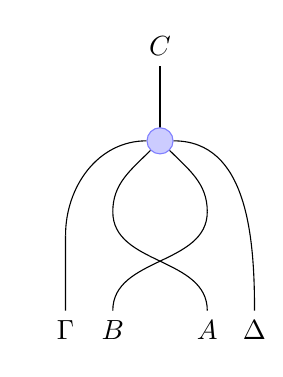
\begin{tikzpicture}[scale=0.6,auto]
\node (gamma) at (-2,-4) {$\Gamma$};
\node (a) at (1,-4) {$A$};
\node (b) at (-1,-4) {$B$};
\node (delta) at (2,-4) {$\Delta$};
\node (top) at (0,2) {$C$};
\draw (0,0) -- (top);
\bluenode (o) at (0,0) {};
\draw[out=90,in=180] (-2,-2) to (o);
\draw (gamma) -- (-2,-2);
\draw[out=90,in=225] (-1,-1.5) to (o);
\draw[out=90,in=270] (a) to (-1,-1.5);
\draw[out=90,in=315] (1,-1.5) to (o);
\draw[out=90,in=270] (b) to (1,-1.5);
\draw[out=90,in=0] (delta) to (o);
\end{tikzpicture}
&
\tagarray{\label{deduction_rule_ex}}
\end{tabular}
\end{center}

% Cut rule ======
\begin{center}
\begin{tabular}{ >{\centering}m{6cm} >{\centering}m{6cm} >{\centering}m{2cm}}
\AxiomC{$\Gamma \vdash A$} 
\AxiomC{$A, \Delta \vdash B$}
\LeftLabel{(Cut): }
\RightLabel{\scriptsize cut}
\BinaryInfC{$\Gamma, \Delta \vdash B$}
\DisplayProof
&
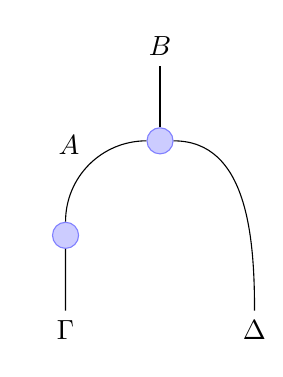
\begin{tikzpicture}[scale=0.6,auto]
\node (top) at (0,4) {$B$};
\node (bottoml) at (-2,-2) {$\Gamma$};
\node (bottomr) at (2,-2) {$\Delta$};
\bluenode (1) at (-2,0) {};
\bluenode (2) at (0,2) {};
\draw (bottoml) -- (1);
\draw[out=90,in=180] (1) to node {$A$} (2);
\draw[out=90,in=0] (bottomr) to (2);
\draw (2) -- (top);
\end{tikzpicture}
&
\tagarray{\label{deduction_rule_cut}}
\end{tabular}
\end{center}


% Right tensor ======
\begin{center}
\begin{tabular}{ >{\centering}m{6cm} >{\centering}m{6cm} >{\centering}m{2cm}}
\AxiomC{$\Gamma \vdash A$} \AxiomC{$\Delta \vdash B$}
\LeftLabel{(Right $\otimes$): }
\RightLabel{\scriptsize $\otimes$-$R$}
\BinaryInfC{$\Gamma, \Delta \vdash A \otimes B$}
\DisplayProof
&
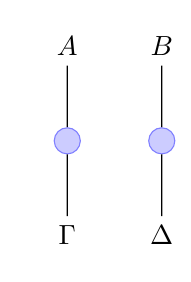
\begin{tikzpicture}[scale=0.6,auto]
\node (topl) at (-1,2) {$A$};
\node (topr) at (1,2) {$B$};
\node (bottoml) at (-1,-2) {$\Gamma$};
\node (bottomr) at (1,-2) {$\Delta$};
\bluenode (l) at (-1,0) {};
\bluenode (r) at (1,0) {};
\draw (bottoml) -- (l);
\draw (l) -- (topl);
\draw (bottomr) -- (r);
\draw (r) -- (topr);
\end{tikzpicture}
&
\tagarray{\label{deduction_rule_righttensor}}
\end{tabular}
\end{center}

% Left tensor ======
\begin{center}
\begin{tabular}{ >{\centering}m{6cm} >{\centering}m{6cm} >{\centering}m{2cm}}
\AxiomC{$\Gamma, A, B \vdash C$}
\LeftLabel{(Left $\otimes$): }
\RightLabel{\scriptsize $\otimes$-$L$}
\UnaryInfC{$\Gamma, A \otimes B \vdash C$}
\DisplayProof
&
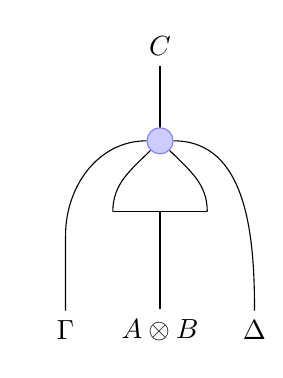
\begin{tikzpicture}[scale=0.6,auto]
\node (gamma) at (-2,-4) {$\Gamma$};
\node (mid) at (0,-4) {$A \otimes B$};
\node (delta) at (2,-4) {$\Delta$};
\node (top) at (0,2) {$C$};
\draw (0,0) -- (top);
\bluenode (o) at (0,0) {};
\draw[out=90,in=180] (-2,-2) to (o);
\draw (gamma) -- (-2,-2);
\draw (-1,-1.5) to (1,-1.5);
\draw[out=90,in=225] (-1,-1.5) to (o);
\draw (mid) to (0,-1.5);
\draw[out=90,in=315] (1,-1.5) to (o);
\draw[out=90,in=0] (delta) to (o);
\end{tikzpicture}
&
\tagarray{\label{deduction_rule_lefttensor}}
\end{tabular}
\end{center}

% Right Hom ======
\begin{center}
\begin{tabular}{ >{\centering}m{6cm} >{\centering}m{6cm} >{\centering}m{2cm}}
\AxiomC{$A, \Gamma \vdash B$}
\LeftLabel{(Right $\multimap$): }
\RightLabel{\scriptsize $\multimap R$ }
\UnaryInfC{$\Gamma \vdash A \multimap B$}
\DisplayProof
&
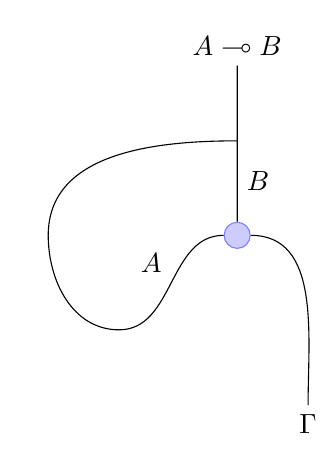
\begin{tikzpicture}[scale=0.6,auto]
\node (topr) at (1,4) {$A \multimap B$};
\bluenode (o) at (1,0) {};
\node (gamma) at (2.5,-4) {$\Gamma$};
\draw[out=90,in=0] (gamma) to (o);
\draw[out=0,in=180] (-1.5,-2) to node {$A$} (o);
\draw[out=180,in=270] (-1.5,-2) to (-3,0);
\draw[out=90,in=180] (-3,0) to (1,2);
\draw (o) to node [swap] {$B$} (1,2);
\draw (1,2) to (topr);
\end{tikzpicture}
&
\tagarray{\label{deduction_rule_righthom}}
\end{tabular}
\end{center}

% Left Hom ======
\begin{center}
\begin{tabular}{ >{\centering}m{6cm} >{\centering}m{6cm} >{\centering}m{2cm}}
\AxiomC{$\Gamma \vdash A$} \AxiomC{$B, \Delta \vdash C$}
\LeftLabel{(Left $\multimap$): }
\RightLabel{\scriptsize $\multimap L$ }
\BinaryInfC{$\Gamma, A \multimap B, \Delta \vdash C$}
\DisplayProof
&
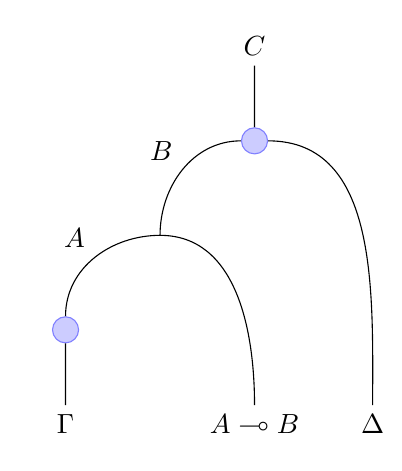
\begin{tikzpicture}[scale=0.6,auto]
\node (topr) at (1,2) {$C$};
\bluenode (q) at (-3,-4) {};
\bluenode (o) at (1,0) {};
\node (delta) at (3.5,-6) {$\Delta$};
\node (gamma) at (-3, -6) {$\Gamma$};
\node (ab) at (1,-6) {$A \multimap B$};
\draw[out=90,in=0] (delta) to (o);
\draw (o) to (topr);
\draw[out=90,in=180] (-1,-2) to node {$B$} (o);
\draw[out=90,in=270] (gamma) to (q);
\draw[out=90,in=180] (q) to node {$A$} (-1,-2);
\draw[out=90,in=0] (ab) to (-1,-2);
\end{tikzpicture}
&
\tagarray{\label{deduction_rule_lefthom}}
\end{tabular}
\end{center}

% Promotion ======
\begin{center}
\begin{tabular}{ >{\centering}m{6cm} >{\centering}m{6cm} >{\centering}m{2cm}}
\AxiomC{$! \Gamma \vdash A$}
\LeftLabel{(Promotion): }
\RightLabel{\scriptsize prom}
\UnaryInfC{$!\Gamma \vdash !A$}
\DisplayProof
&
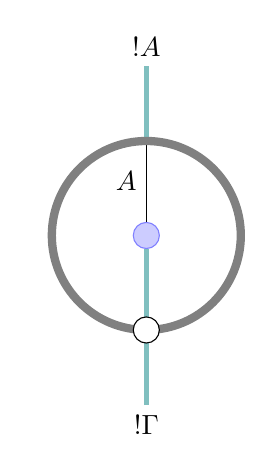
\begin{tikzpicture}[scale=0.6,auto]
\node (top) at (0,4) {$!A$};
\node (bottom) at (0,-4) {$!\Gamma$};
\bluenode (o) at (0,0) {};
\draw (o) to node {$A$} (0,2);
\drawbang (bottom) -- (0,-2);
\drawbang (0,2) -- (top);
\drawbang (0,-2) -- (o);
\drawprom (0,0) ellipse (2cm and 2cm);
\dernode (bottom) at (0,-2) {};
\end{tikzpicture}
&
\tagarray{\label{deduction_rule_prom}}
\end{tabular}
\end{center}

% Dereliction ======
\begin{center}
\begin{tabular}{ >{\centering}m{6cm} >{\centering}m{6cm} >{\centering}m{2cm}}
\AxiomC{$\Gamma, A \vdash B$}
\LeftLabel{(Dereliction): }
\RightLabel{\scriptsize der}
\UnaryInfC{$\Gamma, !A \vdash B$}
\DisplayProof
&
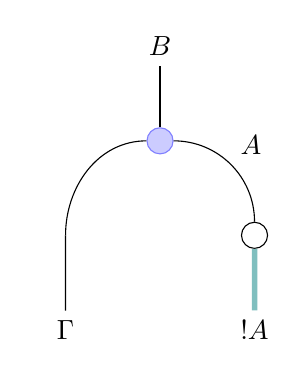
\begin{tikzpicture}[scale=0.6,auto]
\node (top) at (0,2) {$B$};
\bluenode (o) at (0,0) {};
\dernode (d) at (2,-2) {};
\node (gamma) at (-2, -4) {$\Gamma$};
\node (banga) at (2,-4) {$!A$};
\drawbang (banga) -- (d);
\draw (o) -- (top);
\draw[out=90,in=0] (d) to node [swap] {$A$} (o);
\draw (gamma) to (-2,-2);
\draw[out=90,in=180] (-2,-2) to (o);
\end{tikzpicture}
&
\tagarray{\label{deduction_rule_der}}
\end{tabular}
\end{center}

% Contraction ======
\begin{center}
\begin{tabular}{ >{\centering}m{6cm} >{\centering}m{6cm} >{\centering}m{2cm}}
\AxiomC{$\Gamma, !A, !A \vdash B$}
\LeftLabel{(Contraction): }
\RightLabel{\scriptsize ctr}
\UnaryInfC{$\Gamma, !A \vdash B$}
\DisplayProof
&
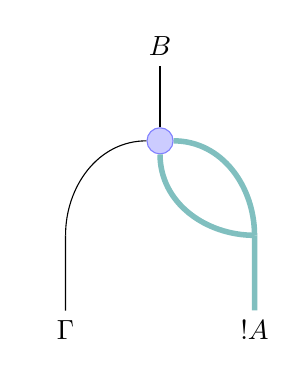
\begin{tikzpicture}[scale=0.6,auto]
\node (top) at (0,2) {$B$};
\bluenode (o) at (0,0) {};
\node (gamma) at (-2, -4) {$\Gamma$};
\node (banga) at (2,-4) {$!A$};
\drawbang (banga) -- (2,-2);
\draw (o) -- (top);
\drawbang[out=90,in=0] (2,-2) to (o);
\drawbang[out=180,in=270] (2,-2) to (o);
\draw (gamma) to (-2,-2);
\draw[out=90,in=180] (-2,-2) to (o);
\end{tikzpicture}
&
\tagarray{\label{deduction_rule_contr}}
\end{tabular}
\end{center}

% Weakening ======
\begin{center}
\begin{tabular}{ >{\centering}m{6cm} >{\centering}m{6cm} >{\centering}m{2cm}}
\AxiomC{$\Gamma \vdash B$}
\LeftLabel{(Weakening): }
\RightLabel{\scriptsize weak}
\UnaryInfC{$\Gamma, !A \vdash B$}
\DisplayProof
&
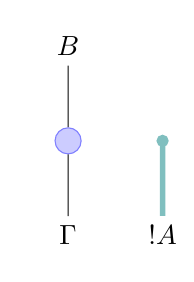
\begin{tikzpicture}[scale=0.6,auto]
\node (topl) at (-1,2) {$B$};
\node (bottoml) at (-1,-2) {$\Gamma$};
\node (bottomr) at (1,-2) {$!A$};
\bluenode (l) at (-1,0) {};
\draw (bottoml) -- (l);
\draw (l) -- (topl);
\drawbang (bottomr) -- (1,0);
\node[circle,draw=teal!50,fill=teal!50,inner sep=0.5mm] at (1,0) {};
\end{tikzpicture}
&
\tagarray{\label{deduction_rule_weak}}
\end{tabular}
\end{center}

% Left 1 ======
\begin{center}
\begin{tabular}{ >{\centering}m{6cm} >{\centering}m{6cm} >{\centering}m{2cm}}
\AxiomC{$\Gamma \vdash A$}
\LeftLabel{(Left $1$): }
\RightLabel{\scriptsize $1$-$L$}
\UnaryInfC{$\Gamma, 1 \vdash A$}
\DisplayProof
&
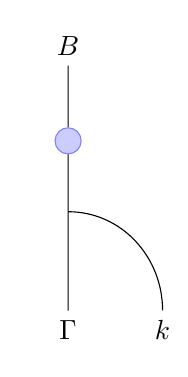
\begin{tikzpicture}[scale=0.6,auto]
\node (topl) at (-1,3) {$B$};
\node (bottoml) at (-1,-3) {$\Gamma$};
\node (bottomr) at (1,-3) {$k$};
\bluenode (l) at (-1,1) {};
\draw (bottoml) -- (l);
\draw (l) -- (topl);
\draw[out=90,in=0] (bottomr) to (-1,-0.5);
\end{tikzpicture}
&
\tagarray{\label{deduction_rule_left1}}
\end{tabular}
\end{center}

% Right 1 ======
\begin{center}
\begin{tabular}{ >{\centering}m{6cm} >{\centering}m{6cm} >{\centering}m{2cm}}
\AxiomC{}
\LeftLabel{(Right $1$): }
\RightLabel{\scriptsize $1$-$R$}
\UnaryInfC{$\vdash 1$}
\DisplayProof
&
\begin{tikzpicture}[scale=0.6,auto]
\node (top) at (0,1) {$k$};
\node (bottom) at (0,-1) {$k$};
\draw (bottom) -- (top);
\end{tikzpicture}
&
\tagarray{\label{deduction_rule_right1}}
\end{tabular}
\end{center}

For the examples in this paper, the relevant deduction rules are the axiom rule, the cut rule, the right and left $\multimap$ introduction rules, the contraction rule and the promotion and dereliction rules. With the exception of the last two, the others have the same form as the rules in classical logic, except with $\multimap$ instead of $\Rightarrow$ and with the contraction rule restricted to formulas ${!} A$. For more on classical versus linear logic, see Remark \ref{remark:embedding_intuit}.

It is standard practice to use the words \emph{formula} and \emph{type} interchangeably in systems like linear logic, and this is especially convenient when a formula denotes a ``data type'' like integers or lists, as in the following example.

\begin{example}\label{example:first_occur_2} For any type $A$ the type of \emph{integers on $A$} is
\begin{equation}\label{defn:integers} 
\inta_A = {!}( A \multimap A) \multimap (A \multimap A)\,.
\end{equation}
The proof of the linear logic version of the Church numeral $\church{2}$ is
\begin{center}
\AxiomC{}
\UnaryInfC{$A \vdash A$}
\AxiomC{}
\UnaryInfC{$A \vdash A$}
\AxiomC{}
\UnaryInfC{$A \vdash A$}
\RightLabel{\scriptsize$\multimap L$}
\BinaryInfC{$A, A \multimap A \vdash A$}
\RightLabel{\scriptsize$\multimap L$}
\BinaryInfC{$A, A \multimap A, A \multimap A \vdash A$}
\RightLabel{\scriptsize$\multimap R$}
\UnaryInfC{$A \multimap A, A \multimap A \vdash A \multimap A$}
\alwaysDoubleLine
\RightLabel{\scriptsize der}
\UnaryInfC{$!( A \multimap A ), !(A \multimap A) \vdash A \multimap A$}
\alwaysSingleLine
\RightLabel{\scriptsize ctr}
\UnaryInfC{$!( A \multimap A) \vdash A \multimap A$}
\RightLabel{\scriptsize$\multimap R$}
\UnaryInfC{$\vdash \inta_A$}
\DisplayProof
\qquad
\tagarray{\label{church_2_prooftree}}
\end{center}
A doubled horizontal line stands for repeated applications of a deduction rule (in this case, dereliction is applied twice). Although the proof obviously has a structure similar to \eqref{church_2_prooftree_classic} notice that there is a conversion between $A \multimap A$ and its infinite version ${!}(A \multimap A)$, where the duplication occurs. For each integer $n \ge 0$ there is a proof $\church{n}$ of $\inta_A$ constructed along similar lines, see \cite[\S 5.3.2]{girard_llogic} and \cite[\S 3.1]{danos}.
\end{example}

As in intuitionistic logic, cut-elimination in linear logic generates an equivalence relation on proofs of a given sequent, with a unique cut-free proof in each equivalence class. This equivalence relation plays a role similar to diffeomorphism of bordisms in topological field theory, but is more complicated because of the presence of the exponential modality, as for example the diagrammatic transformations in Section \ref{section:cut_elim} below demonstrate. %We will have more to say about cut-elimination for linear logic in Section \ref{section:cut_elim} and Section \ref{section:goi}.

A \emph{categorical semantics} of linear logic \cite{mellies, blue_book} assigns to each type $A$ an object $\den{A}$ of some category and to each proof of $\Gamma \vdash A$ a morphism $\den{\Gamma} \lto \den{A}$ in such a way that two proofs equivalent under cut-elimination are assigned the same morphism; these objects and morphisms are called \emph{denotations}. The connectives of linear logic become structure on the category of denotations, and compatibility with cut-elimination imposes identities relating these structures to one another. The upshot is that to define a categorical semantics the category of denotations must be a closed symmetric monoidal category equipped with a comonad, which is used to model the exponential modality \cite[\S 7]{mellies}. This is a refinement of the equivalence between simply-typed $\lambda$-calculus and cartesian closed categories due to Lambek and Scott \cite{lambek}. The first semantics of linear logic were the coherence spaces of Girard \cite[\S 3]{girard_llogic} which are a refined form of Scott's model of the $\lambda$-calculus. Models of full linear logic with negation involve the $\star$-autonomous categories of Barr \cite{barr_auto,barr_acc,barr_autolin} and the extension to include quantifiers involves indexed monoidal categories \cite{seely}.

In this paper denotations all take place in the category $\cat{V}$ of $k$-vector spaces. We explain the denotations of types now, and leave the denotation of proofs to the next section. To this end, for a vector space $V$ let ${!} V$ denote the cofree cocommutative coalgebra generated by $V$. We will discuss the explicit form of this coalgebra in the next section; for the moment it is enough to know that it exists and is determined up to unique isomorphism.

\begin{definition}\label{defn:denotation_objects} The \emph{denotation} $\den{A}$ of a type $A$ is defined inductively as follows:
\begin{itemize}
\item The propositional variables $x, y, z, \ldots$ are assigned chosen finite-dimensional vector spaces $\den{x}, \den{y}, \den{z}, \ldots$;
\item $\den{1} = k$;
\item $\den{A \otimes B} = \den{A} \otimes \den{B}$;
\item $\den{A \multimap B} = \den{A} \multimap \den{B}$ which is notation for $\Hom_k(\den{A}, \den{B})$;
\item $\den{!A} = {!} \den{A}$.
\end{itemize}
The denotation of a group of formulas $\Gamma = A_1,\ldots,A_n$ is their tensor product
\[
\den{\Gamma} = \den{A_1} \otimes \cdots \otimes \den{A_n}\,.
\]
If $\Gamma$ is empty then $\den{\Gamma} = k$.
\end{definition}

We continue with the Church numeral $\church{2}$ as our motivating example:

\begin{example}\label{example:denotation_2}  Let $A$ be a type whose denotation is $V = \den{A}$. Then from \eqref{defn:integers},
\[
\den{\inta_A} = \den{ {!}( A \multimap A) \multimap (A \multimap A)} = \Hom_k( {!} \End_k(V), \End_k(V) )\,.
\]
Skipping ahead a little, the denotation of the proof $\prf{2}$ of $\vdash \inta_A$ will be a morphism
\begin{equation}\label{eq:2_as_comp_0}
\den{\prf{2}}: k \lto \den{\inta_A} = \Hom_k( {!} \End_k(V), \End_k(V) )\,,
\end{equation}
or equivalently, a linear map ${!} \End_k(V) \lto \End_k(V)$. What is this linear map? It turns out (see Example \ref{example:church_2} below for details) that it is the composite
\begin{equation}\label{eq:2_as_comp}
\xymatrix@C+0.5pc{
{!} \End_k(V) \ar[r]^-{\Delta} & {!} \End_k(V) \otimes {!} \End_k(V) \ar[r]^-{d \otimes d} & \End_k(V)^{\otimes 2} \ar[r]^-{- \circ -} & \End_k(V)
}
\end{equation}
where $\Delta$ is the coproduct, $d$ is the universal map, and the last map is the composition. How to reconcile this linear map with the corresponding program in the $\lambda$-calculus, which has the meaning ``square the input function''? As we will explain below, for $\alpha \in \End_k( V )$ there is a naturally associated element $\ket{o}_\alpha \in {!} \End_k(V)$ with the property that
\[
\Delta \ket{o}_\alpha = \ket{o}_\alpha \otimes \ket{o}_\alpha, \qquad d \ket{o}_\alpha = \alpha\,.
\]
Then $\den{\church{2}}$ maps this element to
\begin{equation}\label{eq:2_deals_with_0}
\ket{o}_\alpha \longmapsto \ket{o}_\alpha \otimes \ket{o}_\alpha \longmapsto \alpha \otimes \alpha \longmapsto \alpha \circ \alpha\,.
\end{equation}
%For $n > 2$ the Church numeral $\church{n}$ has $n$ occurrences of the left $\multimap$ introduction rule, and so has as its leaves $n + 1$ uses of the axiom rule. The corresponding diagram uses the coproduct $n-1$ times, and feeds the results into $n$ derelictions.
This demonstrates how the coalgebra ${!} \End_k(V)$ may be used to encode nonlinear maps, such as squaring an endomorphism.
\end{example}

\begin{remark}\label{remark:embedding_intuit} We have already mentioned the equivalence of the simply-typed $\lambda$-calculus and propositional intuitionistic logic under the Curry-Howard isomorphism \cite[\S 6.5]{selinger}. There is an embedding of propositional intuitionistic logic into propositional intuitionistic \emph{linear} logic \cite[\S 5.1]{girard_llogic} making use of the additive connectives of linear logic which we have omitted in the above. This means that every program in the simply-typed $\lambda$-calculus may be assigned a proof in linear logic (with additives) in such a way that $\beta$-reduction in the $\lambda$-calculus corresponds to cut-elimination in linear logic. For more on linear logic proofs as computer programs, see \cite{lafont,abramsky,benton_etal}.

For example, if $A,B$ denote types in propositional intuitionistic logic, and $A^\circ, B^\circ$ the corresponding types in linear logic, then $(A \Rightarrow B)^\circ := (! A^\circ) \multimap B^\circ$ where for atoms $A$ we declare $A^\circ = A$. There is a corresponding translation of proofs of $\vdash A$ to proofs of $\vdash A^\circ$. The Church numeral $\church{2}$ is a $\lambda$-term of type $(A \rightarrow A) \rightarrow (A \rightarrow A)$ which corresponds to a proof in intuitionistic logic of the sequent $\vdash (A \Rightarrow A) \Rightarrow (A \Rightarrow A)$. If $A$ is atomic, the translation of this type to linear logic is $\inta_A' = {!}( {!}A \multimap A ) \multimap ({!}A \multimap A)$. Thus a Church numeral in the $\lambda$-calculus determines a proof of $\vdash \inta_A'$ not $\vdash \inta_A$ under this translation. However, this translation is not necessarily the most useful or economical one because of the over-use of exponentials \cite[\S 5.3]{girard_llogic}. For reasons of clarity we follow standard practice in using the ``linear logic version'' of the Church numeral $\church{2}$ in Example \ref{example:first_occur_2} above, rather than the literal translation.
\end{remark}

\section{Diagrams and denotations}\label{section:diagrammatics}

In the previous section we introduced the connectives and deduction rules of linear logic, and we associated to each type $A$ a vector space $\den{A}$. In this section we complete the construction of the vector space semantics of linear logic by assigning to each proof $\pi$ of a sequent $\Gamma \vdash B$ a linear map $\den{\Gamma} \lto \den{B}$. We have already sketched how this assignment works in the case of the Church numeral $\church{2}$ in Example \ref{example:denotation_2}.

This is almost completely formal: the category of $k$-vector spaces has all the properties of a category of proof denotations described earlier, including the comonad ${!}$ given by taking cofree cocommutative coalgebras, so it is automatic that semantics of intuitionistic linear logic may be constructed within $\cat{V}$. However, to explicitly calculate the denotations of proofs we need formulas for promotion and dereliction which are not automatic: in fact, this paper seems to be the first time they have been written down. This is not as surprising as it might seem: although studying semantics of \emph{linear} logic using vector spaces is an natural thing to do, research has focused on full linear logic with negation. This is more complicated than the intuitionistic case, because types must be interpreted by self-dual objects and this leads to topological vector spaces \cite{barr_auto, barr_acc, blute,blute_scott,girard_coherentbanach,ehrhard, ehrhard_kothe}.  However these more sophisticated models have the disadvantage that it is inconvenient to write down denotations of proofs, which is why for this introduction we stick to the intuitionistic case. See Remark \ref{remark_otherpromotion} for more on the existing literature.

Our assignment of linear maps to proofs will be presented using string diagrams. One style of string diagrams, called \emph{proof-nets}, were introduced by Girard and have been fundamental to linear logic since the beginning of the subject \cite{girard_llogic}. However proof-nets are designed for full linear logic and this does not match a semantics involving infinite-dimensional vector spaces. Instead we use a style of diagrams which is standard in category theory, following Joyal and Street \cite{JSGoTCI,JSGoTCII,ladia,khovdia}. Our recommended reference for this approach to proof-nets is Melli\`{e}s \cite{mellies, mellies_dia}.
\\

Let $\cat{V}$ denote the category of $k$-vector spaces (not necessarily finite dimensional). Then $\cat{V}$ is symmetric monoidal and for each object $V$ the functor $V \otimes -$ has a right adjoint
\[
V \multimap - := \Hom_k(V, -)\,.
\]
In addition to the usual diagrammatics of a symmetric monoidal category, we draw the counit $V \otimes (V \multimap W) \lto W$ as
\begin{center}
\begin{tabular}{>{\centering}m{5cm} >{\centering}m{1cm}}
\begin{tikzpicture}[scale=0.4,auto]
\node (topr) at (0,3) {$W$};
\coordinate (o) at (0,0) {};
\node (bottoml) at (-3,-4) {$V$};
\node (bottomr) at (3,-4) {$V \multimap W$};
\draw[out=90,in=180] (bottoml) to (o);
\draw[out=90,in=0] (bottomr) to (o);
\draw (o) to (topr);
\end{tikzpicture}
&
\tagarray{\label{eq:adjoint_map_diampee}}
\end{tabular}
\end{center}
The adjoint $Y \lto X \multimap Z$ of a morphism $\phi: X \otimes Y \lto Z$ is depicted as follows:\footnote{This is somewhat against the spirit of the diagrammatic calculus, since the loop labelled $X$ is not ``real'' and is only meant as a ``picture'' to be placed at a vertex between a strand labelled $Y$ and a strand labelled $X \multimap Z$. This should not cause confusion, because we will never manipulate this strand on its own. The idea is that if $X$ were a finite-dimensional vector space, so that $X \multimap Z \cong X^{\vee} \otimes Z$, the above diagram would be absolutely valid, and we persist with the same notation even when $X$ is not dualisable. In our judgement the clarity achieved by this slight cheat justifies a little valour in the face of correctness.}
\begin{center}
\begin{tabular}{>{\centering}m{5cm} >{\centering}m{1cm}}
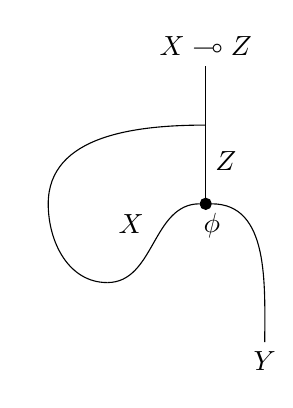
\begin{tikzpicture}[scale=0.5,auto]
\node (topr) at (1,4) {$X \multimap Z$};
\mapnode (o) at (1,0) {};
\node [below] at (o.east) {$\phi$};
\node (gamma) at (2.5,-4) {$Y$};
\draw[out=90,in=0] (gamma) to (o);
\draw[out=0,in=180] (-1.5,-2) to node {$X$} (o);
\draw[out=180,in=270] (-1.5,-2) to (-3,0);
\draw[out=90,in=180] (-3,0) to (1,2);
\draw (o) to node [swap] {$Z$} (1,2);
\draw (1,2) to (topr);
\end{tikzpicture}
&
\tagarray{\label{eq:adjoint_map_diamp}}
\end{tabular}
\end{center}
Next we present the categorical construct corresponding to the exponential modality in terms of an adjunction, following Benton \cite{benton}, see also \cite[\S 7]{mellies}. Let $\cat{C}$ denote the category of counital, coassociative, cocommutative coalgebras in $\cat{V}$. In this paper whenever we say \emph{coalgebra} we mean an object of $\cat{C}$. This is a symmetric monoidal category in which the tensor product (inherited from $\cat{V}$) is cartesian, see \cite[Theorem 6.4.5]{sweedler}, \cite{barr} and \cite[\S 6.5]{mellies}. 

By results of Sweedler \cite[Chapter 6]{sweedler} the forgetful functor $L: \cat{C} \lto \cat{V}$ has a right adjoint $R$ and we set ${!} = L \circ R$, as in the following diagram:\footnote{The existence of a right adjoint to the forgetful functor can also be seen to hold more generally as a consequence of the adjoint functor theorem \cite{barr}.}
\[
\xymatrix@C+3pc{
\cat{C}\ar@<0.7ex>[r]^-{L} & \cat{V} \ar@<0.7ex>[l]^-{R}
}
\qquad
! = L \circ R\,.
\]
Both $L$ and its adjoint $R$ are monoidal functors.

For each $V$ there is a coalgebra $! V$ and a counit of adjunction $d: {!} V \lto V$. Since this map will end up being the interpretation of the dereliction rule in linear logic, we refer to it as the \emph{dereliction map}. In string diagrams it is represented by an empty circle. Although it is purely decorative, it is convenient to represent coalgebras in string diagrams drawn in $\cat{V}$ by thick lines, so that for ${!} V$ the dereliction, coproduct and counit are drawn respectively as follows:
\begin{center}
\begin{tabular}{>{\centering}m{3cm} >{\centering}m{3cm} >{\centering}m{3cm} >{\raggedleft}m{1cm}}
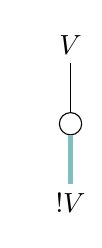
\begin{tikzpicture}[scale=0.5,auto,inner sep=1mm]
\node (top) at (0,2) {$V$};
\dernode (d) at (0,0) {};
\node (banga) at (0,-2) {$!V$};
\drawbang (banga) -- (d);
\draw (d) -- (top);
\end{tikzpicture}
&
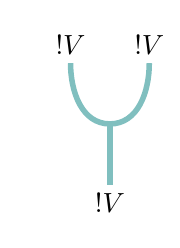
\begin{tikzpicture}[scale=0.5,auto,inner sep=1mm]
\node (topl) at (-1,2) {${!} V$};
\node (topr) at (1,2) {${!} V$};
\coordinate (d) at (0,0);
\node (banga) at (0,-2) {$!V$};
\drawbang (banga) -- (d);
\drawbang[out=0,in=270] (d) to (topr);
\drawbang[out=180,in=270] (d) to (topl);
\end{tikzpicture}
&
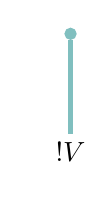
\begin{tikzpicture}[scale=0.5,auto,inner sep=1mm]
\node (banga) at (0,-2) {$!V$};
\node[circle,draw=teal!50,fill=teal!50,inner sep=0.5mm] (blah) at (0,1) {};
\drawbang (banga) -- (blah);
\end{tikzpicture}
&
\tagarray{\label{eq:coalgebra_maps}}
\end{tabular}
\end{center}
In this paper our string diagrams involve both $\cat{V}$ and $\cat{C}$ and our convention is that white regions represent $\cat{V}$ and gray regions stand for $\cat{C}$. A standard way of representing monoidal functors between monoidal categories is using coloured regions \cite[\S 5.7]{mellies}. The image under $L$ of a morphism $\alpha: C_1 \lto C_2$ in $\cat{C}$ is drawn as a vertex in a grey region embedded into a white region. The image of a morphism $\gamma: V_1 \lto V_2$ under $R$ is drawn using a white region embedded in a gray plane. For example, the diagrams representing $L(\alpha), R(\gamma)$ and ${!} \gamma = LR(\gamma)$ are respectively
\begin{center}
\begin{tikzpicture}
[inner sep=0.5mm,scale=0.6,auto,place/.style={circle,draw=blue!50,fill=blue!20,thick},
transition/.style={circle,draw=black,fill=black}]
\node (vtop) at (0,4.5) {$L C_2$};
\node (bottom) at (0,-4.5) {$L C_1$};
\drawbang (top) to (vtop);
\coordinate (bottom_c) at (0,-3);
\drawbang (bottom) to (bottom_c);
\coordinate (top_c) at (0,3);
\draw[color=gray, line width=3pt, fill=gray!20] (0,0) ellipse (2cm and 3cm);
\node (o) at (0,0) [transition] {};
\node [right] at (o.east) {$\alpha$};
\draw (o) to node [swap] {$C_2$} (top_c);
\draw (bottom_c) to node [swap] {$C_1$} (o);
\draw[color=gray, line width=3pt] (0,0) ellipse (2cm and 3cm);
\end{tikzpicture}
\qquad \qquad
\begin{tikzpicture}
[inner sep=0.5mm,scale=0.6,auto,place/.style={circle,draw=blue!50,fill=blue!20,thick},
transition/.style={circle,draw=black,fill=black}]
\draw[color=white,fill=gray!20] (-3,-4.1) rectangle (3,4.1);
\node (vtop) at (0,4.5) {$R V_2$};
\node (bottom) at (0,-4.5) {$R V_1$};
\draw (top) to (vtop);
\coordinate (bottom_c) at (0,-3);
\draw (bottom) to (bottom_c);
\coordinate (top_c) at (0,3);
\draw[color=gray, line width=3pt, fill=white] (0,0) ellipse (2cm and 3cm);
\node (o) at (0,0) [transition] {};
\node [right] at (o.east) {$\gamma$};
\draw (o) to node [swap] {$V_2$} (top_c);
\draw (bottom_c) to node [swap] {$V_1$} (o);
\draw[color=gray, line width=3pt] (0,0) ellipse (2cm and 3cm);
\end{tikzpicture}
\qquad \qquad
\begin{tikzpicture}
[inner sep=0.5mm,scale=0.6,auto,place/.style={circle,draw=blue!50,fill=blue!20,thick},
transition/.style={circle,draw=black,fill=black}]
\node (vtop) at (0,4.5) {${!} V_2 = LR V_2$};
\node (bottom) at (0,-4.5) {${!} V_1 = LR V_1$};
\coordinate (top_c) at (0,3);
\coordinate (bottom_c) at (0,-3);
\drawbang (top) to (vtop);
\drawbang (bottom) to (bottom_c);
\draw[color=gray, line width=3pt, fill=gray!20] (0,0) ellipse (3cm and 3.2cm);
\draw[color=gray, line width=3pt, fill=white] (0,0) ellipse (2.5cm and 1.2cm);
\node (o) at (0,0) [transition] {};
\node [right] at (o.east) {$\gamma$};
\draw (o) to (0,1.2);
\draw (o) to (0,-1.2);
\draw (0,1.2) to node [swap] {$RV_2$} (0,3.2);
\draw (0,-3.2) to node [swap] {$RV_1$} (0,-1.2);
\draw[color=gray, line width=3pt] (0,0) ellipse (3cm and 3.2cm);
\draw[color=gray, line width=3pt] (0,0) ellipse (2.5cm and 1.2cm);
\end{tikzpicture}
\end{center}
The adjunction between $R$ and $L$ means that for any coalgebra $C$ and linear map $\phi: C \lto V$ there is a unique morphism of coalgebras $\Phi : C \lto {!}V$ making
\begin{equation}\label{eq:defining_philift}
\xymatrix@C+1.5pc@R+1.5pc{
C \ar[r]^-{\phi}\ar[dr]_-{\Phi} & V\\
& {!}V \ar[u]_-{d}
}
\end{equation}
commute. The lifting $\Phi$ may be constructed as the unit followed by ${!} \phi$,
\[
\Phi := \xymatrix@C+2pc{ C \ar[r] & {!} C \ar[r]^-{{!} \phi} & {!} V}
\]
and since we use an empty circle to denote the unit $C \lto {!} C$, this has the diagrammatic representation given on the right hand side of the following diagram. The left hand side is a convenient abbreviation for this morphism, that is, for the lifting $\Phi$:
% Promotion ======
\begin{center}
\begin{tabular}{>{\centering}m{3cm} >{\centering}m{1cm} >{\centering}m{5cm} m{1cm}}
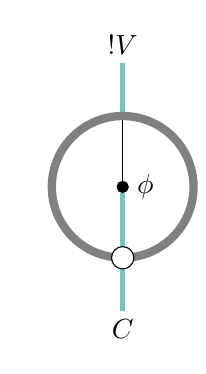
\begin{tikzpicture}[scale=0.6,auto,inner sep=1mm]
\node (top) at (0,3) {$!V$};
\node (bottom) at (0,-3) {$C$};
\mapnode (o) at (0,0) {};
\node [right] at (o.east) {$\phi$};
\draw (o) to (0,2);
\drawbang (bottom) -- (0,-1.5);
\drawbang (0,1.5) -- (top);
\drawbang (0,-1.5) -- (o);
\drawprom (0,0) ellipse (1.5cm and 1.5cm);
\dernode (bottom) at (0,-1.5) {};
\end{tikzpicture}
& := &
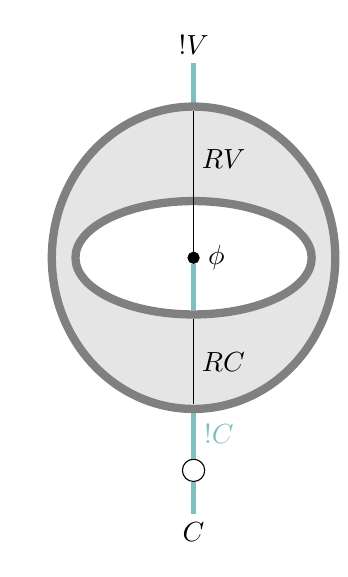
\begin{tikzpicture}[scale=0.6,auto,inner sep=1mm]
\node (vtop) at (0,4.5) {${!} V$};
\node (bottom) at (0,-5.8) {$C$};
\coordinate (top_c) at (0,3);
\coordinate (bottom_c) at (0,-3.2);
\drawbang (top_c) to (vtop);
\dernode (bottomd) at (0,-4.5) {};
\drawbang (bottomd) to node [swap] {${!} C$} (bottom_c);
\drawbang (bottom) to (bottomd);
\draw[color=gray, line width=3pt, fill=gray!20] (0,0) ellipse (3cm and 3.2cm);
\draw[color=gray, line width=3pt, fill=white] (0,0) ellipse (2.5cm and 1.2cm);
\mapnode (o) at (0,0) {};
\node [right] at (o.east) {$\phi$};
\draw (o) to (0,1.2);
\drawbang (o) to (0,-1.1);
\draw (0,1.1) to node [swap] {$RV$} (0,3.1);
\draw (0,-3.1) to node [swap] {$RC$} (0,-1.3);
\end{tikzpicture}
& \tagarray{\label{eq:abbrev_for_prom}}
\end{tabular}
\end{center}
We follow the logic literature in referring to the grey circle denoting the induced map $\Phi$ as a \emph{promotion box}. Commutativity of \eqref{eq:defining_philift} is expressed by the identity
\begin{center}
\begin{tabular}{>{\centering}m{3cm} >{\centering}m{1cm} >{\centering}m{3cm} >{\raggedleft}m{1cm}}
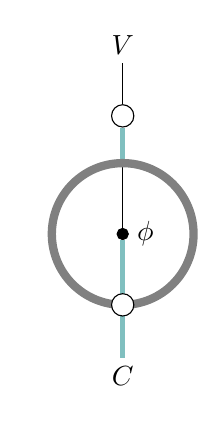
\begin{tikzpicture}[scale=0.6,auto,inner sep=1mm]
\node (top) at (0,4) {$V$};
\dernode (altop) at (0,2.5) {};
\node (bottom) at (0,-3) {$C$};
\mapnode (o) at (0,0) {};
\node [right] at (o.east) {$\phi$};
\draw (o) to (0,2);
\drawbang (bottom) -- (0,-1.5);
\drawbang (0,1.5) -- (altop);
\draw (altop) -- (top);
\drawbang (0,-1.5) -- (o);
\drawprom (0,0) ellipse (1.5cm and 1.5cm);
\dernode (bottom) at (0,-1.5) {};
\end{tikzpicture}
& = &
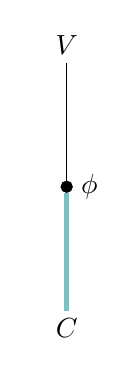
\begin{tikzpicture}[scale=0.6,auto,inner sep=1mm]
\node (top) at (0,3) {$V$};
\node (bottom) at (0,-3) {$C$};
\mapnode (o) at (0,0) {};
\node [right] at (o.east) {$\phi$};
\drawbang (bottom) -- (o);
\draw (o) -- (top);
\end{tikzpicture}
& \tagarray{\label{eq:prom_cancel_der}}
\end{tabular}
\end{center}

The coalgebra ${!} V$ and the dereliction map ${!} V \lto V$ satisfy a universal property and are therefore unique up to isomorphism. However, to actually understand the denotations of proofs, we will need the more explicit construction which follows from the work of Sweedler \cite{sweedler} and is spelt out in \cite{murfet_coalg}. If $V$ is finite-dimensional then
\begin{equation}\label{eq:presentation_intro}
{!} V = \bigoplus_{P \in V} \Sym_P(V)
\end{equation}
where $\Sym_P(V) = \Sym(V)$ is the symmetric coalgebra. If $e_1,\ldots,e_n$ is a basis for $V$ then as a vector space $\Sym(V) \cong k[e_1,\ldots,e_n]$. The notational convention in \cite{murfet_coalg} is to denote, for elements $\nu_1,\ldots,\nu_s \in V$, the corresponding tensor in $\Sym_P(V)$ using kets
\begin{equation}\label{eq:ket_notation}
\ket{\nu_1,\ldots,\nu_s}_P := \nu_1 \otimes \cdots \otimes \nu_s \in \Sym_P(V)\,.
\end{equation}
And in particular, the identity element of $\Sym_P(V)$ is denoted by a vacuum vector
\begin{equation}\label{eq:vacuum}
\ket{o}_P := 1 \in \Sym_P(V)\,.
\end{equation}
We remark that if $\nu = 0$ then $\ket{\nu}_P = 0$ is the zero vector, which is distinct from $\ket{o}_P = 1$. We keep in mind that \eqref{eq:vacuum} denotes the case $s = 0$ of \eqref{eq:ket_notation} and to avoid unwieldy notation we sometimes write $\nu_1 \otimes \cdots \otimes \nu_s \cdot \ket{o}_P$ for $\ket{\nu_1,\ldots,\nu_s}_P$. With this notation the universal map $d: {!} V \lto V$ is defined by
\[
d \ket{o}_P = P, \quad d\ket{\nu}_P = \nu, \quad d\ket{\nu_1,\ldots,\nu_s}_P = 0 \quad s > 1\,.
\]
The coproduct on ${!} V$ is defined by
\begin{equation}\label{eq:lc_coalgebra_1}
\Delta \ket{ \nu_1, \ldots, \nu_s }_P = \sum_{I \subseteq \{ 1, \ldots, s \}} \ket{ \nu_I }_P \otimes \ket{ \nu_{I^c} }_P
\end{equation}
where $I$ ranges over all subsets including the empty set, for a subset $I = \{ i_1, \ldots, i_p \}$ we denote by $\nu_I$ the sequence $\nu_{i_1},\ldots,\nu_{i_p}$, and $I^c$ is the complement of $I$. In particular
\[
\Delta \ket{o}_P = \ket{o}_P \otimes \ket{o}_P\,.
\]
The counit ${!} V \lto k$ is defined by $\ket{o}_P \mapsto 1$ and $\ket{\nu_1,\ldots,\nu_s}_P \mapsto 0$ for $s > 0$.

When $V$ is infinite-dimensional we may define ${!} V$ as the direct limit over the coalgebras ${!} W$ for finite-dimensional subspaces $W \subseteq V$. These are sub-coalgebras of ${!} V$, and we may therefore use the same notation as in \eqref{eq:ket_notation} to denote arbitrary elements of ${!} V$. Moreover the coproduct, counit and universal map $d$ are given by the same formulas; see \cite[\S 2.1]{murfet_coalg}. A proof of the fact that the map $d: {!} V \lto V$ described above is universal among linear maps to $V$ from cocommutative coalgebras is given in \cite[Theorem 2.18]{murfet_coalg}, but as has been mentioned this is originally due to Sweedler \cite{sweedler}, see \cite[Appendix B]{murfet_coalg}.

To construct semantics of linear logic we also need an explicit description of liftings, as given by the next theorem which is \cite[Theorem 2.20]{murfet_coalg}. For a set $X$ the set of partitions of $X$ is denoted $\cat{P}_X$.

\begin{theorem}\label{theorem:describe_lifting} Let $W, V$ be vector spaces and $\phi: {!}W \lto V$ a linear map. The unique lifting to a morphism of coalgebras $\Phi: {!}W \lto {!}V$ is given by
\begin{equation}\label{eq:describe_lift}
\Phi \ket{ \nu_1, \ldots, \nu_s }_P = \sum_{C \in \cat{P}_{\{1,\ldots,s\}}} \phi \ket{ \nu_{C_{1}} }_P \otimes \cdots \otimes \phi \ket{ \nu_{C_{l}} }_P \cdot \ket{o}_Q
\end{equation}
for $P, \nu_1,\ldots,\nu_s \in W$, where $Q = \phi \ket{o}_P$ and $l$ denotes the length of the partition $C$.
\end{theorem}

%In constructing the vector space semantics of linear logic we will only encounter \eqref{eq:abbrev_for_prom} in the case where $C = {!} W$. %We will however give examples of lifting that involve other coalgebras, including the next example and in Appendix \ref{section:example_lifting}.

\begin{example}\label{example:lifting_trivial} The simplest example of a coalgebra is the field $k$. Any $P \in V$ determines a linear map $k \lto V$ whose lifting to a morphism of coalgebras $k \lto {!}V$ sends $1 \in k$ to the vacuum $\ket{o}_P$, as shown in the commutative diagram
\begin{equation}\label{eq:kaiwanxiao}
\xymatrix@C+2pc{
k \ar[r]^-{P} \ar@{.>}[dr]_-{\ket{o}_P} & V\\
& ! V \ar[u]_-{d}
}\,.
\end{equation}
Such liftings arise from promotions with empty premises, e.g. the proof
\begin{center}
\AxiomC{}
\UnaryInfC{$A \vdash A$}
\RightLabel{\scriptsize $\multimap R$}
\UnaryInfC{$\vdash A \multimap A$}
\RightLabel{\scriptsize prom}
\UnaryInfC{$\vdash {!}(A \multimap A)$}
\DisplayProof
\end{center}
Incidentally, this explains why $\den{!A} = \Sym(\den{A})$ does not lead to semantics of linear logic, since the denotation of the above proof is a morphism of coalgebras $k \lto {!} \End_k(\den{A})$ whose composition with dereliction yields the map $k \lto \End_k( \den{A} )$ sending $1 \in k$ to the identity. But this map does not admit a lifting into the symmetric coalgebra, because it produces an infinite sum. However the symmetric coalgebra \emph{is} universal in a restricted sense and is (confusingly) sometimes also called a cofree coalgebra; see \cite[\S 4]{quillen}. For further discussion of the symmetric coalgebra in the context of linear logic see \cite{blute_fock,mellies2}.
\end{example}

\subsection{The vector space semantics}\label{section:vector_space_sem}

Recall from Definition \ref{defn:denotation_objects} the definition of $\den{A}$ for each type $A$.

\begin{definition}\label{defn:denotation_morphism} The \emph{denotation} $\den{\pi}$ of a proof $\pi$ of $\Gamma \vdash B$ is a linear map $\den{\Gamma} \lto \den{B}$ defined by inductively assigning a string diagram to each proof tree; by the basic results of the diagrammatic calculus \cite{JSGoTCI} this diagram unambiguously denotes a linear map. The inductive construction is described by the second column in \eqref{deduction_rule_ax} -- \eqref{deduction_rule_weak}. 

In each rule we assume a morphism has already been assigned to each of the sequents in the numerator of the deduction rule. These inputs are represented by blue circles in the diagram, which computes the morphism to be assigned to the denominator. To simplify the appearance of diagrams, we adopt the convention that a strand labelled by a type $A$ represents a strand labelled by the denotation $\den{A}$. In particular, a strand labelled with a sequence $\Gamma = A_1,\ldots,A_n$ represents a strand labelled by $\den{A_1} \otimes \cdots \otimes \den{A_n}$.
\end{definition}

Some comments:
\begin{itemize}
\item The diagram for the axiom rule \eqref{deduction_rule_ax} depicts the identity of $\den{A}$.
\item The diagram for the exchange rule \eqref{deduction_rule_ex} uses the symmetry $\den{B} \otimes \den{A} \lto \den{A} \otimes \den{B}$.
\item The diagram for the cut rule \eqref{deduction_rule_cut} depicts the composition of the two inputs.
\item The right tensor rule \eqref{deduction_rule_righttensor} depicts the tensor product of the two given morphisms, while the left tensor rule \eqref{deduction_rule_lefttensor} depicts the identity, viewed as a morphism between two strands labelled $\den{A}$ and $\den{B}$ and a single strand labelled $\den{A} \otimes \den{B}$.
\item The diagram for the right $\multimap$ rule \eqref{deduction_rule_righthom} denotes the adjoint of the input morphism, as explained in \eqref{eq:adjoint_map_diamp}, while the left $\multimap$ rule \eqref{deduction_rule_lefthom} uses the composition map of \eqref{eq:adjoint_map_diampee}.
\item The diagram for the promotion rule \eqref{deduction_rule_prom} depicts the lifting of the input to a morphism of coalgebras, as explained in \eqref{eq:abbrev_for_prom}.
\item The diagram for the dereliction rule \eqref{deduction_rule_der} depicts the composition of the input with the universal map out of the coalgebra ${!} V$. The notation for this map, and the maps in the contraction \eqref{deduction_rule_contr} and weakening rules \eqref{deduction_rule_weak} are as described in \eqref{eq:coalgebra_maps}.
\end{itemize}

\begin{remark} For this to be a valid semantics, two proofs related by cut-elimination must be assigned the same morphism. This is a consequence of the general considerations in \cite[\S 7]{mellies}. More precisely, $\cat{V}$ is a Lafont category \cite[\S 7.2]{mellies} and in the terminology of \emph{loc.cit.} the adjunction between $\cat{V}$ and $\cat{C}$ is a linear-nonlinear adjunction giving rise to a model of intuitionistic linear logic. For an explanation of how the structure of a symmetric monoidal category extrudes itself from the cut-elimination transformations, see \cite[\S 2]{mellies}.
\end{remark}

Given the embedding of the simply-typed $\lambda$-calculus into linear logic, recalled in Remark \ref{remark:embedding_intuit}, and the above construction of an interpretation of linear logic in the category $\cat{V}$ of $k$-vector spaces, we are finally in a position to answer Question \ref{question:lambda} in the positive. With patience, the reader may use the above to translate any program into a linear map. To explain how this works in practice, we go through the details of assigning a diagram and the corresponding linear map to the proof tree \eqref{church_2_prooftree} of the Church numeral $\church{2}$. 

\begin{example}\label{example:church_2} We convert the proof tree \eqref{church_2_prooftree} to a diagram in stages, beginning with the leaves. Each stage is depicted in three columns: in the first is a partial proof tree, in the second is the diagram assigned to it by Definition \ref{defn:denotation_morphism}, and in the third is the explicit linear map which is the value of the diagram. 

Recall that a strand labelled $A$ actually stands for the vector space $V = \den{A}$, so for instance the first diagram denotes a linear map $V \otimes \End_k(V) \lto V$:
\begin{center}
% Church numeral 2 layer 1
\begin{tabular}{>{\centering}m{6cm} >{\centering}m{5cm} >{\centering}m{4cm}}
\AxiomC{}
\UnaryInfC{$A \vdash A$}
\AxiomC{}
\UnaryInfC{$A \vdash A$}
\RightLabel{\scriptsize$\multimap L$}
\BinaryInfC{$A, A \multimap A \vdash A$}
\DisplayProof
&
\begin{tikzpicture}[scale=0.3,auto]
\node (topr) at (0,2) {$A$};
\coordinate (o) at (0,0);
\node (delta) at (2.5,-4) {$A \multimap A$};
\node (left) at (-2.5, -4) {$A$};
\draw (o) to (topr);
\draw[out=90,in=180] (left) to (o);
\draw[out=90,in=0] (delta) to (o);
\end{tikzpicture}
&
$a \otimes \alpha \mapsto \alpha(a)$
\end{tabular}
\end{center}
\begin{center}
% Church numeral 2 layer 2
\begin{tabular}{>{\centering}m{6cm} >{\centering}m{5cm} >{\centering}m{4cm}}
\AxiomC{}
\UnaryInfC{$A \vdash A$}
\AxiomC{}
\UnaryInfC{$A \vdash A$}
\AxiomC{}
\UnaryInfC{$A \vdash A$}
\RightLabel{\scriptsize$\multimap L$}
\BinaryInfC{$A, A \multimap A \vdash A$}
\RightLabel{\scriptsize$\multimap L$}
\BinaryInfC{$A, A \multimap A, A \multimap A \vdash A$}
\DisplayProof
&
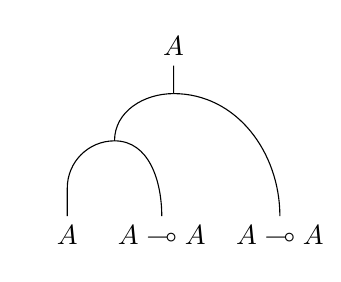
\begin{tikzpicture}[scale=0.3,auto]
\node (topr) at (1.5,2) {$A$};
\coordinate (q) at (-3,-4);
\coordinate (o) at (1.5,0);
\node (delta) at (6,-6) {$A \multimap A$};
\node (gamma) at (-3, -6) {$A$};
\node (ab) at (1,-6) {$A \multimap A$};
\draw[out=90,in=0] (delta) to (o);
\draw (o) to (topr);
\draw[out=90,in=180] (-1,-2) to (o);
\draw[out=90,in=270] (gamma) to (q);
\draw[out=90,in=180] (q) to (-1,-2);
\draw[out=90,in=0] (ab) to (-1,-2);
\end{tikzpicture}
&
$a \otimes \alpha \otimes \beta \mapsto \beta( \alpha(a) )$
\end{tabular}
\end{center}

\begin{center}
% Church numeral 2 layer 3
\begin{tabular}{ >{\centering}m{6cm} >{\centering}m{5cm} >{\centering}m{4cm}}
\AxiomC{}
\UnaryInfC{$A \vdash A$}
\AxiomC{}
\UnaryInfC{$A \vdash A$}
\AxiomC{}
\UnaryInfC{$A \vdash A$}
\RightLabel{\scriptsize$\multimap L$}
\BinaryInfC{$A, A \multimap A \vdash A$}
\RightLabel{\scriptsize$\multimap L$}
\BinaryInfC{$A, A \multimap A, A \multimap A \vdash A$}
\RightLabel{\scriptsize$\multimap R$}
\UnaryInfC{$A \multimap A, A \multimap A \vdash A \multimap A$}
\DisplayProof
&
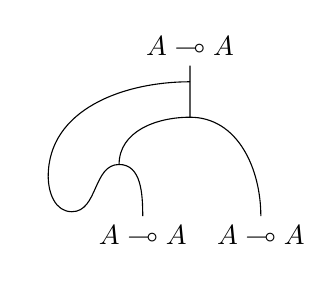
\begin{tikzpicture}[scale=0.3,auto]
\coordinate (o) at (2,0);
\node (top) at ($ (o) + (0,3) $) {$A \multimap A$}; % coordinates are relative to (o)

\coordinate (left_meet) at ($ (o) - (3, 2) $);
\draw[out=90,in=180] (left_meet) to (o);

% Coproduct and derelictions
\node (R) at ($ (o) + (3,-5) $) {$A \multimap A$};
\node (L) at ($ (o) + (-2,-5) $) {$A \multimap A$};
\coordinate (delta) at ($ (o) - (0,5) $);
\draw[out=90,in=0] (R) to (o);

% The A line curl from bottom to top
\coordinate (left_curve) at ($ (o) - (5, 4) $);
\coordinate (left_curve_mid) at ($ (o) - (6,2.5) $);
\coordinate (first_meeting_top) at ($ (o) + (0,1.5) $);
\draw[out=90,in=0] (L) to (left_meet);
\draw[out=0,in=180] (left_curve) to (left_meet);
\draw (o) to (first_meeting_top);
\draw[out=180,in=270] (left_curve) to (left_curve_mid);
\draw[out=90,in=180] (left_curve_mid) to (first_meeting_top);

\draw (first_meeting_top) to (top);
\end{tikzpicture}
&
$\alpha \otimes \beta \mapsto \beta \circ \alpha$
\end{tabular}
\end{center}

\begin{center}
% TIKZ Church numeral 2 layer 4
\begin{tabular}{ >{\centering}m{6cm} >{\centering}m{6cm} >{\centering}m{1cm}}
\AxiomC{}
\UnaryInfC{$A \vdash A$}
\AxiomC{}
\UnaryInfC{$A \vdash A$}
\AxiomC{}
\UnaryInfC{$A \vdash A$}
\RightLabel{\scriptsize$\multimap L$}
\BinaryInfC{$A, A \multimap A \vdash A$}
\RightLabel{\scriptsize$\multimap L$}
\BinaryInfC{$A, A \multimap A, A \multimap A \vdash A$}
\RightLabel{\scriptsize$\multimap R$}
\UnaryInfC{$A \multimap A, A \multimap A \vdash A \multimap A$}
\alwaysDoubleLine
\RightLabel{\scriptsize der}
\UnaryInfC{$!( A \multimap A ), !(A \multimap A) \vdash A \multimap A$}
\alwaysSingleLine
\DisplayProof
&
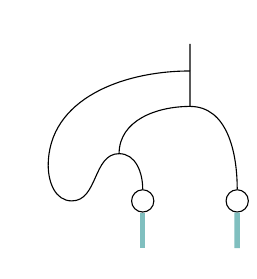
\begin{tikzpicture}[scale=0.3,auto,inner sep=1mm]
\coordinate (o) at (2,0);
\node (top) at ($ (o) + (0,3) $) {}; % coordinates are relative to (o)

\coordinate (left_meet) at ($ (o) - (3, 2) $);
\draw[out=90,in=180] (left_meet) to (o);

% Coproduct and derelictions
\dernode (R) at ($ (o) + (2,-4) $) {};
\dernode (L) at ($ (o) + (-2,-4) $) {};
\coordinate (delta) at ($ (o) - (0,5) $);
\draw[out=90,in=0] (R) to (o);
\drawbang (R) to ($ (R) - (0,2) $);
\drawbang (L) to ($ (L) - (0,2) $);

% The A line curl from bottom to top
\coordinate (left_curve) at ($ (o) - (5, 4) $);
\coordinate (left_curve_mid) at ($ (o) - (6,2.5) $);
\coordinate (first_meeting_top) at ($ (o) + (0,1.5) $);
\draw[out=90,in=0] (L) to (left_meet);
\draw[out=0,in=180] (left_curve) to (left_meet);
\draw (o) to (first_meeting_top);
\draw[out=180,in=270] (left_curve) to (left_curve_mid);
\draw[out=90,in=180] (left_curve_mid) to (first_meeting_top);

\draw (first_meeting_top) to (top);
\end{tikzpicture}
&

\tagarray{\label{2_prime_pre}}

\end{tabular}
\end{center}
The map ${!} \End_k(V) \otimes {!} \End_k(V) \lto \End_k(V)$ in \eqref{2_prime_pre} is zero on $\ket{\nu_1,\ldots,\nu_s}_\alpha \otimes \ket{\mu_1,\ldots,\mu_t}_\beta$ for $\alpha,\beta \in \End_k(V)$ unless $s,t \le 1$, and in those cases it is given by
\begin{align*}
\ket{o}_\alpha \otimes \ket{o}_\beta &\longmapsto \beta \circ \alpha\\
\ket{\nu}_\alpha \otimes \ket{o}_\beta &\longmapsto \beta \circ \nu\\
\ket{o}_\alpha \otimes \ket{\mu}_\beta &\longmapsto \mu \circ \alpha\\
\ket{\nu}_\alpha \otimes \ket{\mu}_\beta &\longmapsto \mu \circ \nu\,.
\end{align*}
The next deduction rule in $\church{2}$ is a contraction:
\begin{center}
% TIKZ Church numeral 2 layer 4
\begin{tabular}{ >{\centering}m{6cm} >{\centering}m{6cm} >{\centering}m{1cm}}
\AxiomC{}
\UnaryInfC{$A \vdash A$}
\AxiomC{}
\UnaryInfC{$A \vdash A$}
\AxiomC{}
\UnaryInfC{$A \vdash A$}
\RightLabel{\scriptsize$\multimap L$}
\BinaryInfC{$A, A \multimap A \vdash A$}
\RightLabel{\scriptsize$\multimap L$}
\BinaryInfC{$A, A \multimap A, A \multimap A \vdash A$}
\RightLabel{\scriptsize$\multimap R$}
\UnaryInfC{$A \multimap A, A \multimap A \vdash A \multimap A$}
\alwaysDoubleLine
\RightLabel{\scriptsize der}
\UnaryInfC{$!( A \multimap A ), !(A \multimap A) \vdash A \multimap A$}
\alwaysSingleLine
\RightLabel{\scriptsize ctr}
\UnaryInfC{$!( A \multimap A ) \vdash A \multimap A$}
\DisplayProof
&
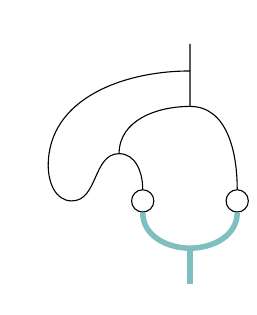
\begin{tikzpicture}[scale=0.3,auto,inner sep=1mm]
\coordinate (o) at (2,0);
\node (top) at ($ (o) + (0,3) $) {}; % coordinates are relative to (o)

\coordinate (left_meet) at ($ (o) - (3, 2) $);
\draw[out=90,in=180] (left_meet) to (o);

% Coproduct and derelictions
\dernode (R) at ($ (o) + (2,-4) $) {};
\dernode (L) at ($ (o) + (-2,-4) $) {};
\coordinate (delta) at ($ (o) - (0,6) $);
\draw[out=90,in=0] (R) to (o);
\drawbang[out=270,in=0] (R) to (delta);
\drawbang[out=270,in=180] (L) to (delta);
\drawbang (delta) to ($ (delta) - (0,1.5) $);

% The A line curl from bottom to top
\coordinate (left_curve) at ($ (o) - (5, 4) $);
\coordinate (left_curve_mid) at ($ (o) - (6,2.5) $);
\coordinate (first_meeting_top) at ($ (o) + (0,1.5) $);
\draw[out=90,in=0] (L) to (left_meet);
\draw[out=0,in=180] (left_curve) to (left_meet);
\draw (o) to (first_meeting_top);
\draw[out=180,in=270] (left_curve) to (left_curve_mid);
\draw[out=90,in=180] (left_curve_mid) to (first_meeting_top);

\draw (first_meeting_top) to (top);
\end{tikzpicture}

&

\tagarray{\label{2_prime}}
\end{tabular}
\end{center}
The denotation of this map is the composition $\phi = \den{\church{2}}: {!} \End_k(V) \lto \End_k(V)$ in \eqref{eq:2_as_comp}. We may compute using the above that 
\begin{equation}\label{eq:church_2_den}
\phi \ket{o}_\alpha = \alpha^2, \qquad \phi \ket{\nu}_\alpha = \{ \nu, \alpha \}\,, \qquad \phi \ket{\nu\mu}_\alpha = \{ \nu, \mu \}\,.
\end{equation}
For example
\begin{gather*}
\ket{\nu}_\alpha \longmapsto \ket{\nu}_\alpha \otimes \ket{o}_\alpha + \ket{o}_\alpha \otimes \ket{\nu}_\alpha \longmapsto \alpha \circ \nu + \nu \circ \alpha = \{ \nu, \alpha \}\,.
\end{gather*}
The final step in the proof of $\church{2}$ consists of moving the ${!}(A \multimap A)$ to the right side of the sequent, which yields the final diagram:
% TIKZ ----- Church numeral 2
\begin{center}
\begin{tabular}{ >{\centering}m{8cm} >{\centering}m{3cm}}
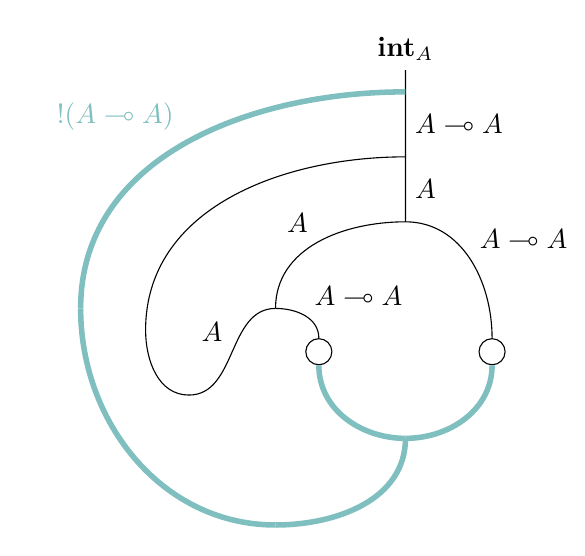
\begin{tikzpicture}[scale=0.55,auto]
\coordinate (o) at (2,0);
\node (top) at ($ (o) + (0,4) $) {$\inta_A$}; % coordinates are relative to (o)

\coordinate (left_meet) at ($ (o) - (3, 2) $);
\draw[out=90,in=180] (left_meet) to node {$A$} (o);

% Coproduct and derelictions
\dernode (R) at ($ (o) + (2,-3) $) {};
\dernode (L) at ($ (o) + (-2,-3) $) {};
\coordinate (delta) at ($ (o) - (0,5) $);
\draw[out=90,in=0] (R) to node [swap] {$A \multimap A$} (o);
\drawbang[out=0,in=270] (delta) to (R);
\drawbang[out=180,in=270] (delta) to (L);

% The A line curl from bottom to top
\coordinate (left_curve) at ($ (o) - (5, 4) $);
\coordinate (left_curve_mid) at ($ (o) - (6,2.5) $);
\coordinate (first_meeting_top) at ($ (o) + (0,1.5) $);
\draw[out=90,in=0] (L) to node [swap] {$A \multimap A$} (left_meet);
\draw[out=0,in=180] (left_curve) to node {$A$} (left_meet);
\draw (o) to node [swap] {$A$} (first_meeting_top);
\draw[out=180,in=270] (left_curve) to (left_curve_mid);
\draw[out=90,in=180] (left_curve_mid) to (first_meeting_top);

\coordinate (second_meeting_top) at ($ (first_meeting_top) + (0,1.5) $);
\draw (first_meeting_top) to node [swap] {$A \multimap A$} (second_meeting_top);
\draw (second_meeting_top) to (top);

\coordinate (curve_bottom) at ($ (left_meet) - (0,5) $);
\coordinate (curve_left) at ($ (o) - (7.5, 2) $);
\drawbang[out=0,in=270] (curve_bottom) to (delta);
\drawbang[out=180,in=270] (curve_bottom) to (curve_left);
\drawbang[out=90,in=180] (curve_left) to node {$!(A \multimap A)$} (second_meeting_top);
\end{tikzpicture}
&
\tagarray{\label{church_2_diagram}}
\end{tabular}
\end{center}
% End Church numeral 2
The denotation of this morphism is the map in \eqref{eq:2_as_comp_0}. The reader might like to compare this style of diagram for $\church{2}$ to the corresponding proof-net in \cite[\S 5.3.2]{girard_llogic}. 
\end{example}

In Example \ref{example:denotation_2} we sketched how to recover the function $\alpha \mapsto \alpha^2$ from the denotation of the Church numeral $\church{2}$, but now we can put this on a firmer footing. The translation of the $\lambda$-calculus into linear logic encourages us to think of a proof $\pi$ of a sequent $! B \vdash C$ as a program whose input of type $B$ may be used multiple times. There is \emph{a priori} no linear map $\den{B} \lto \den{C}$ associated to $\pi$ but there is a function $\den{\pi}_{nl}$ defined on $P \in \den{B}$ by lifting to $! \den{B}$ and then applying $\den{\pi}$:
\begin{equation}\label{eq:lifting_vacua}
\xymatrix@C+2pc{
k \ar[r]^-{P} \ar@{.>}[dr]_-{\ket{o}_P} & \den{B} & \den{C}\\
& ! \den{B} \ar[u]_-{d} \ar[ur]_-{\den{\pi}}
}\,.
\end{equation}
%We saw an example of this pattern in Example \ref{example:church_2}.
That is,

\begin{definition}\label{defn:nonlinear_denotation}
The function $\den{\pi}_{nl}: \den{B} \lto \den{C}$ is defined by $\den{\pi}_{nl}(P) = \den{\pi} \ket{o}_P$.
\end{definition}

The discussion above shows that, with $V = \den{A}$,

\begin{lemma}\label{lemma:nonlinear_recover} $\den{\church{2}}_{nl}: \End_k(V) \lto \End_k(V)$ is the map $\alpha \mapsto \alpha^2$.
\end{lemma}

This completes our explanation of how to represent the Church numeral $\church{2}$ as a linear map (modulo the evasion discussed in Remark \ref{remark_otherpromotion}). From this presentation we see clearly that the non-linearity of the map $\alpha \mapsto \alpha^2$ is concentrated, in fact, not in the duplication step but in the ``promotion'' step \eqref{eq:lifting_vacua} where the input vector $\alpha$ is turned into a vacuum $\ket{o}_\alpha \in {!} \End_k(V)$. The promotion step is non-linear since $\ket{o}_\alpha + \ket{o}_\beta$ is not a morphism of coalgebras and thus cannot be equal to $\ket{o}_{\alpha + \beta}$. After this step, the duplication, dereliction and composition shown in \eqref{eq:2_deals_with_0} are all linear. Finally, when $k = \mathbb{C}$ it is interesting to compare $\den{2}_{nl}$ with the map $\alpha \mapsto \alpha^2$ of smooth manifolds $\End_k(V)$, see Appendix \ref{section:example_lifting}.

%(see the discussion of tangents in Appendix \ref{section:example_lifting}) 

\begin{example}\label{example:2_promotion} Let $\church{2}'$ denote the proof of ${!}(A \multimap A) \vdash A \multimap A$ in \eqref{2_prime}. As discussed in Example \ref{example:denotation_2}, we may confuse the denotation of $\church{2}$ and $\church{2}'$. Applied to $\church{2}'$ the promotion rule generates a new proof,
\begin{prooftree}
\AxiomC{$\church{2}'$}
\noLine\UnaryInfC{$\vdots$}
\def\extraVskip{5pt}
\noLine\UnaryInfC{$!(A \multimap A) \vdash A \multimap A$}
\def\extraVskip{2pt}
\RightLabel{\scriptsize prom}
\UnaryInfC{$!( A \multimap A) \vdash {!}(A \multimap A)$}
\end{prooftree}
which we denote $\operatorname{prom}( \church{2}' )$. By definition the denotation $\Phi := \den{ \operatorname{prom}( \church{2}' ) }$ of this proof is the unique morphism of coalgebras
\[
\Phi: {!} \End_k(V) \lto {!} \End_k(V)
\]
with the property that $d \circ \Phi = \phi$, where $\phi = \den{\church{2}}$ is as in \eqref{eq:2_as_comp}. From \eqref{eq:church_2_den} and Theorem \ref{theorem:describe_lifting} we compute that, for example
\begin{align*}
\Phi \ket{o}_\alpha &= \ket{o}_{\alpha^2}\,,\\
\Phi \ket{\nu}_\alpha &= \{ \nu, \alpha \} \cdot \ket{o}_{\alpha^2},\\
\Phi \ket{\nu \mu}_\alpha &= \big( \{ \nu, \mu \} + \{ \nu, \alpha \} \otimes \{ \mu, \alpha \} \big) \cdot \ket{o}_{\alpha^2}\,,\\
\Phi \ket{\nu \mu \theta}_\alpha &= \big( \{ \nu, \mu \} \otimes \{ \theta, \alpha \} + \{ \theta, \mu \} \otimes \{ \nu, \alpha \} + \{ \nu, \theta \} \otimes \{ \mu, \alpha \}\\
&+ \{ \nu, \alpha \} \otimes \{ \mu, \alpha \} \otimes \{ \theta, \alpha \} \big) \cdot \ket{o}_{\alpha^2}\,.
\end{align*}
Note that the commutators, e.g. $\{ \nu, \alpha \}$ are defined using the product internal to $\End_k(V)$, whereas inside the bracket in the last two lines, the terms $\{ \nu, \alpha \}$ and $\{ \mu, \alpha \}$ are multiplied in the algebra $\Sym( \End_k(V) )$ before being made to act on the vacuum.
\end{example}

%The approach we have chosen has the advantage of being universal in a certain sense: given another categorical semantics, say in a closed symmetric monoidal category $\cat{T}$ with comonad $Q$ modelling the exponential, if there is a strong monoidal functor $F: \cat{T} \lto \cat{V}$ (e.g. the objects of $\cat{T}$ are vector spaces with additional structure) then for any object $V \in \cat{T}$ the morphism $QV \lto V$ becomes a map $FQV \lto FV$, and since $FQV$ is a coalgebra, this factors as
%\[
%\xymatrix@C+1.5pc@R+1.5pc{
%FQV \ar[r]\ar[dr] & FV\\
%& {!}FV \ar[u]_-{d}
%}
%\]
%In this way it is possible to relate semantics such as Ehrhard's finiteness spaces \cite{ehrhard} to the ``universal'' semantics defined above.
\begin{remark}\label{remark_otherpromotion} As we have already mentioned, there are numerous other semantics of linear logic defined using topological vector spaces. The reader curious about how these vector space semantics are related to the ``relational'' style of semantics such as coherence spaces should consult Ehrhard's paper on finiteness spaces \cite{ehrhard}.

Indeed one can generate numerous examples of vector space semantics by looking at comonads on the category $\cat{V}$ defined by truncations on the coalgebras ${!} V$. For example, given a vector space $V$, let ${!}_0 V$ denote the subspace of ${!} V$ generated by the vacua $\ket{o}_P$. This is the free space on the underlying \emph{set} of $V$, and it is a subcoalgebra of ${!} V$ given as a coproduct of trivial coalgebras. It is easy to see that this defines an appropriate comonad and gives rise to a semantics of linear logic \cite[\S 4.3]{valiron}. However the semantics defined using ${!} V$ is more interesting, because universality allows us to mix in arbitrary coalgebras $C$. In Appendix \ref{section:example_lifting} we examine the simplest example where $C$ is the dual of the algebra $k[t]/t^2$ and relate this to tangent vectors.
\end{remark}

\section{Cut-elimination}\label{section:cut_elim}

We have now introduced the sequent calculus of intuitionistic linear logic, and seen how to represent linear logic in vector spaces. But so far we have only talked about denotations of types and proofs which, to borrow an insightful analogy from \cite[\S III]{girard_towards}, together play a role analogous to that of statics within classical mechanics. The \emph{dynamical} part of linear logic is a set of rewrite rules on proofs in the sequent calculus, which together define the possible ``interactions'' between proofs and the results of these interactions. The full set of rewrite rules is given in \cite[Section 3]{mellies} and in the alternative language of proof-nets in \cite[\S 4]{girard_llogic}, \cite[p.18]{pagani}. To help the reader grasp the core idea, we present a worked example involving our favourite proof $\church{2}$ where we give both the rewrites and the associated transformations of string diagrams.

A proof in linear logic is \emph{cut-free} if it contains no occurrences of the cut rule. For each sequent $\Gamma \vdash A$ there is an equivalence relation on the set of proofs of the sequent, generated by a series of proof transformations that are together called \emph{cut-elimination}. Each of these transformations generates a proof that is ``closer'' to being cut-free, according to a certain measure of cut complexity.

\begin{theorem}[Girard] Every proof in linear logic may be related via cut-elimination to a unique cut-free proof of the same sequent.
\end{theorem}
\begin{proof}
See \cite[Chapter 13]{girard_prooftypes} for a sketch of Gentzen's cut-elimination in classical logic, and \cite[\S 3]{mellies} for the case of intuitionistic linear logic.
\end{proof}

Given a proof $\pi$ the unique cut-free proof in the same equivalence class is called the \emph{cut-free normalisation} of $\pi$. Before the main example, we examine two proof transformations from the list in \cite[Section 3]{mellies} which will be needed.

\begin{example}\label{example:cut_elim_examples} The cut-elimination transformation \cite[\S 3.11.10]{mellies} tells us that
\begin{center}
\begin{tabular}{ >{\centering}m{7cm} >{\centering}m{4cm} >{\centering}m{3cm}}
\AxiomC{$\pi_1$}
\noLine\UnaryInfC{$\vdots$}
\def\extraVskip{5pt}
\noLine\UnaryInfC{$\Gamma \vdash A$}
\def\extraVskip{2pt}
\AxiomC{$\pi_2$}
\noLine\UnaryInfC{$\vdots$}
\def\extraVskip{5pt}
\noLine\UnaryInfC{$B, A \vdash C$}
\def\extraVskip{2pt}
\RightLabel{\scriptsize $\multimap R$}
\UnaryInfC{$A \vdash B \multimap C$}
\RightLabel{\scriptsize cut}
\BinaryInfC{$\Gamma \vdash B \multimap C$}
\DisplayProof
&
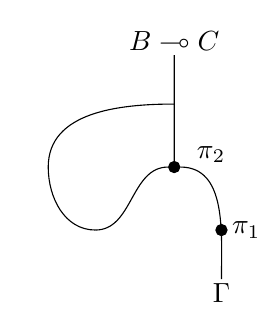
\begin{tikzpicture}[inner sep = 0.5mm, scale=0.4,auto]
\node (topr) at (1,4) {$B \multimap C$};
\node[circle,draw=black,fill=black] (o) at (1,0) {};
\node [above] at (o.east) {$\;\;\;\;\;\;\;\;\den{\pi_2}$};
\node[circle,draw=black,fill=black] (other) at (2.5,-2) {};
\node [right] at (other.east) {$\den{\pi_1}$};
\node (gamma) at (2.5,-4) {$\Gamma$};
\draw[out=90,in=0] (gamma) to (o);
\draw[out=0,in=180] (-1.5,-2) to (o);
\draw[out=180,in=270] (-1.5,-2) to (-3,0);
\draw[out=90,in=180] (-3,0) to (1,2);
\draw (o) to (1,2);
\draw (1,2) to (topr);
\end{tikzpicture}
&
\tagarray{\label{eq:cutelim1}}
\end{tabular}
\end{center}
is transformed to the proof
\begin{center}
\begin{tabular}{ >{\centering}m{7cm} >{\centering}m{4cm} >{\centering}m{3cm}}
\AxiomC{$\pi_1$}
\noLine\UnaryInfC{$\vdots$}
\def\extraVskip{5pt}
\noLine\UnaryInfC{$\Gamma \vdash A$}
\def\extraVskip{2pt}
\AxiomC{$\pi_2$}
\noLine\UnaryInfC{$\vdots$}
\def\extraVskip{5pt}
\noLine\UnaryInfC{$B, A \vdash C$}
\def\extraVskip{2pt}
\RightLabel{\scriptsize cut}
\BinaryInfC{$B, \Gamma \vdash C$}
\RightLabel{\scriptsize $\multimap R$}
\UnaryInfC{$\Gamma \vdash B \multimap C$}
\DisplayProof
&
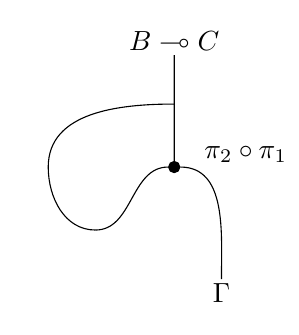
\begin{tikzpicture}[inner sep = 0.5mm, scale=0.4,auto]
\node (topr) at (1,4) {$B \multimap C$};
\node[circle,draw=black,fill=black] (o) at (1,0) {};
\node [above] at (o.east) {$\;\;\;\;\;\;\;\;\;\;\;\;\;\;\;\;\;\den{\pi_2} \circ \den{\pi_1}$};
\node (gamma) at (2.5,-4) {$\Gamma$};
\draw[out=90,in=0] (gamma) to (o);
\draw[out=0,in=180] (-1.5,-2) to (o);
\draw[out=180,in=270] (-1.5,-2) to (-3,0);
\draw[out=90,in=180] (-3,0) to (1,2);
\draw (o) to (1,2);
\draw (1,2) to (topr);
\end{tikzpicture}
&
\tagarray{\label{eq:cutelim2}}
\end{tabular}
\end{center}
and thus the two corresponding diagrams are equal. In this case, the equality generated by cut-elimination expresses the fact that the Hom-tensor adjunction is natural.

The transformation \cite[\S 3.8.2]{mellies} tells us that
\begin{center}
\begin{tabular}{ >{\centering}m{7cm} >{\centering}m{4cm} >{\centering}m{3cm}}
\AxiomC{$\pi_2$}
\noLine\UnaryInfC{$\vdots$}
\def\extraVskip{5pt}
\noLine\UnaryInfC{$A \vdash B$}
\def\extraVskip{2pt}
\RightLabel{\scriptsize $\multimap R$}
\UnaryInfC{$\vdash A \multimap B$}
\AxiomC{$\pi_1$}
\noLine\UnaryInfC{$\vdots$}
\def\extraVskip{5pt}
\noLine\UnaryInfC{$\Gamma \vdash A$}
\def\extraVskip{2pt}
\AxiomC{$\pi_3$}
\noLine\UnaryInfC{$\vdots$}
\def\extraVskip{5pt}
\noLine\UnaryInfC{$B \vdash C$}
\def\extraVskip{2pt}
\RightLabel{\scriptsize $\multimap L$}
\BinaryInfC{$\Gamma, A \multimap B \vdash C$}
\RightLabel{\scriptsize cut}
\BinaryInfC{$\Gamma \vdash C$}
\DisplayProof
&
\begin{tikzpicture}[scale=0.35,auto]
\node (top) at (0,5) {$C$};
\mapnode (mid_top) at (0,2) {};
\node [above] at (mid_top.east) {$\;\;\;\;\;\;\den{\pi_3}$};
\node (bottoml) at (-3,-5) {$\Gamma$};
\mapnode (pi1) at (-3,-3) {};
\node [above] at (pi1.east) {$\;\;\;\;\;\;\;\;\;\den{\pi_1}$};
\coordinate (o) at (0,0);
\draw (o) -- (mid_top);
\draw (mid_top) -- (top);
\draw (bottoml) -- (pi1);
\draw[out=90,in=180] (pi1) to (o);
\mapnode (other) at (3,-3) {};
\coordinate (other_up) at (3,-2) {};
\node [right] at (other.east) {$\den{\pi_2}$};
\draw[out=90,in=0] (other_up) to (o);
\draw (other) to (other_up);
\coordinate (turn) at ($ (other) - (1.5,2) $);
\coordinate (upper_turn) at ($ (turn) + (-1,1) $);
\draw[out=270,in=0] (other) to (turn);
\draw[out=180,in=270] (turn) to (upper_turn);
\draw[out=90,in=180] (upper_turn) to (other_up);
\end{tikzpicture}
&
\tagarray{\label{eq:cutelim3}}
\end{tabular}
\end{center}
may be transformed to
\begin{center}
\begin{tabular}{ >{\centering}m{8cm} >{\centering}m{3cm} >{\centering}m{3cm}}
\AxiomC{$\pi_1$}
\noLine\UnaryInfC{$\vdots$}
\def\extraVskip{5pt}
\noLine\UnaryInfC{$\Gamma \vdash A$}
\def\extraVskip{2pt}
\AxiomC{$\pi_2$}
\noLine\UnaryInfC{$\vdots$}
\def\extraVskip{5pt}
\noLine\UnaryInfC{$A \vdash B$}
\def\extraVskip{2pt}
\RightLabel{\scriptsize cut}
\BinaryInfC{$\Gamma \vdash B$}
\AxiomC{$\pi_3$}
\noLine\UnaryInfC{$\vdots$}
\def\extraVskip{5pt}
\noLine\UnaryInfC{$B \vdash C$}
\def\extraVskip{2pt}
\RightLabel{\scriptsize cut}
\BinaryInfC{$\Gamma \vdash C$}
\DisplayProof
&
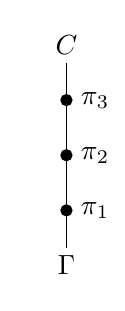
\begin{tikzpicture}[scale=0.35,auto,inner sep=1mm]
\node (top) at (0,5) {$C$};
\mapnode (pi3) at (0,3) {};
\node [right] at (pi3.east) {$\den{\pi_3}$};
\mapnode (pi2) at (0,1) {};
\node [right] at (pi2.east) {$\den{\pi_2}$};
\mapnode (pi1) at (0,-1) {};
\node [right] at (pi1.east) {$\den{\pi_1}$};
\node (bottom) at (0,-3) {$\Gamma$};
\draw (bottom) -- (pi1);
\draw (pi1) -- (pi2);
\draw (pi2) -- (pi3);
\draw (pi3) -- (top);
\end{tikzpicture}
&
\tagarray{\label{eq:cutelim4}}
\end{tabular}
\end{center}
which is again an obvious property of the Hom-tensor adjunction.
\end{example}

The following proof $\prf{\mathrm{mult}}_2$ represents multiplication by $2$ on $A$-integers:
\begin{center}
% TIKZ Church numeral 2 layer 4
\begin{tabular}{ >{\centering}m{9cm} >{\centering}m{6cm}}
\AxiomC{$\church{2}'$}
\noLine\UnaryInfC{$\vdots$}
\def\extraVskip{5pt}
\noLine\UnaryInfC{$!(A \multimap A) \vdash A \multimap A$}
\def\extraVskip{2pt}
\RightLabel{\scriptsize prom}
\UnaryInfC{$!( A \multimap A) \vdash {!}(A \multimap A)$}
\AxiomC{}
\UnaryInfC{$A \multimap A \vdash A \multimap A$}
\RightLabel{\scriptsize$\multimap L$}
\BinaryInfC{$!(A \multimap A), \inta_A \vdash A \multimap A$}
\RightLabel{\scriptsize$\multimap R$}
\UnaryInfC{$\inta_A \vdash \inta_A$}
\DisplayProof
&
% TIKZ ---- picture of mult_2
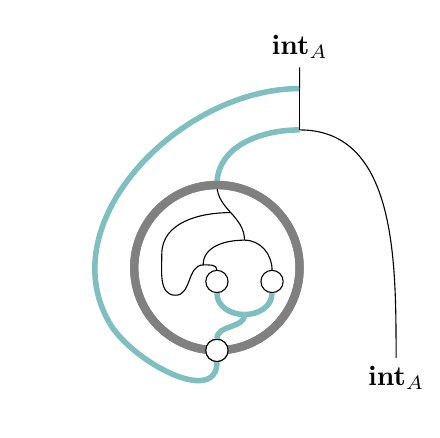
\begin{tikzpicture}[scale=0.35,auto,inner sep=1mm]
\coordinate (topr) at (0,2);
\coordinate (comp) at (3,4);
\drawbang[out=90,in=180] (topr) to (comp);
\drawprom (0,-1) ellipse (3cm and 3cm);
\dernode (bottomr) at (0,-4) {};

% -------- promoted 2 ---------
% All coordinates are relative to the composition vertex (o), which itself
% has its coordinates derived from topr. This is the only link to the outside namespace.
\coordinate (o) at ($ (topr) + (1,-2) $);
\coordinate (ellipse_center) at ($ (o) - (1,1) $);
\coordinate (elbow) at ($ (o) - (3, 0.5) $);
\coordinate (top_of_circle) at ($ (o) + (-1,2) $);
\draw[out=90,in=270] (o) to (top_of_circle);
\drawprom (ellipse_center) ellipse (3cm and 3cm); % outer boundary
\dernode (bottomr) at ($ (o) - (1,4) $) {};
\dernode (R) at ($ (o) + (1, -1.5) $) {}; % right dereliction
\dernode (L) at ($ (o) - (1,1.5) $) {}; % left dereliction
\coordinate (left_curve) at ($ (o) - (2.5,2) $);
\coordinate (left_meet) at ($ (o) - (1.5, 0.9) $);
\coordinate (delta) at ($ (o) - (0, 2.7) $); % coproduct vertex
\draw[out=90,in=0] (R) to node [swap] {} (o);
\drawbang[out=0,in=270] (delta) to (R);
\drawbang[out=180,in=270] (delta) to (L);
\drawbang[out=90,in=270] (bottomr) to (delta);
\draw[out=90,in=180] (left_meet) to (o);
\draw[out=90,in=0] (L) to (left_meet);
\draw[out=0,in=180] (left_curve) to (left_meet);
\draw[out=180,in=270] (left_curve) to (elbow);
\draw[out=90,in=180] (elbow) to ($ (o)!.5!(top_of_circle) $);
% ------ end promoted 2 ------

% Now for the rest of the diagram
\coordinate (curve) at (-3.9, -3);
\coordinate (meet) at (3,5.5);
\drawbang[out=300,in=270] (curve) to (bottomr);
\drawbang[out=120,in=180] (curve) to (meet);
\node (inta) at (6.5,-5) {$\inta_A$};
\draw[out=90,in=0] (inta) to (comp);
\node (vtop) at (3,7) {$\inta_A$};
\draw (meet) to (vtop);
\draw (comp) to (meet);
\end{tikzpicture}
\end{tabular}
\end{center}
where $\church{2}'$ is the proof in \eqref{2_prime}. We feed $\church{2}$ as input to $\prf{\mathrm{mult}}_2$ by cutting:
\begin{center}
\begin{tabular}{ >{\centering}m{6cm} >{\centering}m{6cm} >{\centering}m{4cm}}
\AxiomC{$\church{2}$}
\noLine\UnaryInfC{$\vdots$}
\def\extraVskip{5pt}
\noLine\UnaryInfC{$\vdash \inta_A$}
\def\extraVskip{2pt}
\AxiomC{$\prf{\mathrm{mult}}_2$}
\noLine\UnaryInfC{$\vdots$}
\def\extraVskip{5pt}
\noLine\UnaryInfC{$\inta_A \vdash \inta_A$}
\def\extraVskip{2pt}
\RightLabel{\scriptsize cut}
\BinaryInfC{$\vdash \inta_A$}
\DisplayProof
&
% TIKZ ---- picture of mult_2
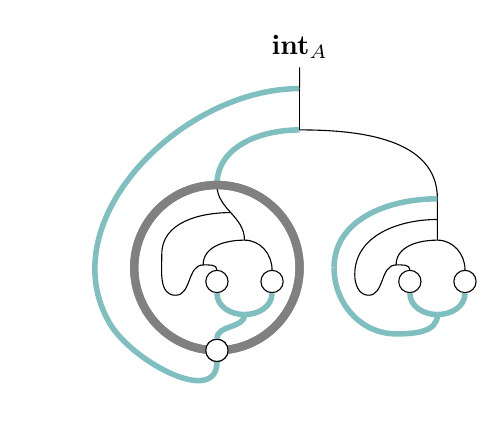
\begin{tikzpicture}[scale=0.35,auto,inner sep=1mm]
\coordinate (topr) at (0,2);
\coordinate (comp) at (3,4);
\drawbang[out=90,in=180] (topr) to (comp);
\drawprom (0,-1) ellipse (3cm and 3cm);
\dernode (bottomr) at (0,-4) {};

% -------- promoted 2 ---------
% All coordinates are relative to the composition vertex (o), which itself
% has its coordinates derived from topr. This is the only link to the outside namespace.
\coordinate (o) at ($ (topr) + (1,-2) $);
\coordinate (ellipse_center) at ($ (o) - (1,1) $);
\coordinate (elbow) at ($ (o) - (3, 0.5) $);
\coordinate (top_of_circle) at ($ (o) + (-1,2) $);
\draw[out=90,in=270] (o) to (top_of_circle);
\drawprom (ellipse_center) ellipse (3cm and 3cm); % outer boundary
\dernode (bottomr) at ($ (o) - (1,4) $) {};
\dernode (R) at ($ (o) + (1, -1.5) $) {}; % right dereliction
\dernode (L) at ($ (o) - (1,1.5) $) {}; % left dereliction
\coordinate (left_curve) at ($ (o) - (2.5,2) $);
\coordinate (left_meet) at ($ (o) - (1.5, 0.9) $);
\coordinate (delta) at ($ (o) - (0, 2.7) $); % coproduct vertex
\draw[out=90,in=0] (R) to node [swap] {} (o);
\drawbang[out=0,in=270] (delta) to (R);
\drawbang[out=180,in=270] (delta) to (L);
\drawbang[out=90,in=270] (bottomr) to (delta);
\draw[out=90,in=180] (left_meet) to (o);
\draw[out=90,in=0] (L) to (left_meet);
\draw[out=0,in=180] (left_curve) to (left_meet);
\draw[out=180,in=270] (left_curve) to (elbow);
\draw[out=90,in=180] (elbow) to ($ (o)!.5!(top_of_circle) $);
% ------ end promoted 2 ------

% Now for the rest of the diagram
\coordinate (curve) at (-3.9, -3);
\coordinate (meet) at (3,5.5);
\drawbang[out=300,in=270] (curve) to (bottomr);
\drawbang[out=120,in=180] (curve) to (meet);
\node (vtop) at (3,7) {$\inta_A$};
\draw (meet) to (vtop);
\draw (comp) to (meet);

% ----------The Church 2 on the right
\coordinate (2o) at ($ (topr) + (8,-2) $);

\coordinate (2left_meet) at ($ (2o) - (1.5, 0.9) $);
\draw[out=90,in=180] (2left_meet) to (2o);

% Coproduct and derelictions
\dernode (2R) at ($ (2o) + (1,-1.5) $) {};
\dernode (2L) at ($ (2o) + (-1,-1.5) $) {};
\coordinate (2delta) at ($ (2o) - (0,2.7) $);
\draw[out=90,in=0] (2R) to (2o);
\drawbang[out=0,in=270] (2delta) to (2R);
\drawbang[out=180,in=270] (2delta) to (2L);

% The A line curl from bottom to top
\coordinate (2left_curve) at ($ (2o) - (2.5, 2) $);
\coordinate (2left_curve_mid) at ($ (2o) - (3,1.25) $);
\coordinate (2first_meeting_top) at ($ (2o) + (0,0.75) $);
\draw[out=90,in=0] (2L) to (2left_meet);
\draw[out=0,in=180] (2left_curve) to (2left_meet);
\draw[out=180,in=270] (2left_curve) to (2left_curve_mid);

\coordinate (2curve_bottom) at ($ (2left_meet) - (0,2.5) $);
\coordinate (2curve_left) at ($ (2o) - (3.75, 1) $);
\drawbang[out=0,in=270] (2curve_bottom) to (2delta);
\drawbang[out=180,in=270] (2curve_bottom) to (2curve_left);


% the lines from the right 2 to the comp vertex are scaled along the line
\coordinate (2top) at ($ (2o) + (0,1.5) $);
\draw[out=90,in=0] (2top) to (comp);
\draw (2o) to (2top);
\drawbang[out=90,in=180] (2curve_left) to (2top);
\draw[out=90,in=180] (2left_curve_mid) to ($ (2o)!.5!(2top) $);
\end{tikzpicture}

&

\tagarray{\label{cut_mult_2}}
\end{tabular}
\end{center}
We denote this cut of the two proofs by $\prf{\mathrm{mult}}_2 \l \church{2}$. Not surprisingly, the cut-free normalisation of $\prf{\mathrm{mult}}_2 \l \church{2}$ is the Church numeral $\church{4}$. Each of the proof transformations generated by the cut-elimination algorithm applied to $\prf{\mathrm{mult}}_2 \l \church{2}$ (see below) yields a new proof with the same denotation, and this sequence of proofs represents a particular sequence of manipulations of the string diagram. 

We now enumerate these diagrammatic transformations. From \eqref{cut_mult_2} the first step is to use naturality of the Hom-tensor adjunction, as in the manipulation from \eqref{eq:cutelim1} to \eqref{eq:cutelim2}. Then we are in the position of \eqref{eq:cutelim3}, with $\pi_2$ a part of $\church{2}$ and $\pi_1$ the promoted Church numeral. The manipulation from \eqref{eq:cutelim3} to \eqref{eq:cutelim4} is to take the left leg and feed it as an input to the right leg. This yields the first equality below. The second equality follows from the fact that a promotion box represents a morphism of coalgebras, and thus can be commuted past the coproduct whereby it is duplicated:
\begin{center}
% TIKZ picture ---- stacked 2 promotions LEFT
\begin{tabular}{m{0.8cm} m{0.3cm} m{4cm} m{0.3cm} m{6cm} m{1cm}}
\eqref{cut_mult_2} & = &
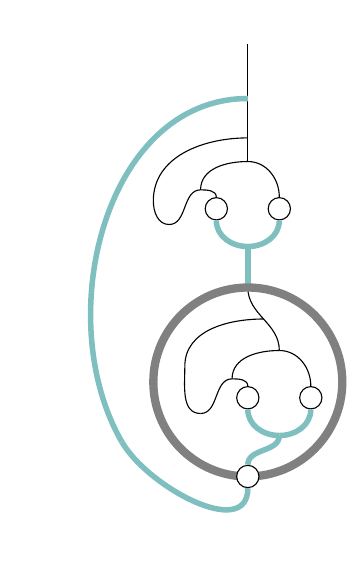
\begin{tikzpicture}[scale=0.4,auto,inner sep=1mm]
\coordinate (topr) at (0,2); % top of the bottom promoted 2
\coordinate (curve) at (-4, -2.9);
%\coordinate (comp) at (0,4) {};
\node (vtop) at ($ (topr) + (0,8) $) {};
\coordinate (meet) at ($ (vtop) - (0,2) $); % where the curved !( A -o A ) arc meets at the top

\draw (meet) to (vtop);

% ----------The Church 2 on the right
\coordinate (2o) at ($ (topr) + (0,4) $);
\coordinate (2left_meet) at ($ (2o) - (1.5, 0.9) $);
\draw[out=90,in=180] (2left_meet) to (2o);

% Coproduct and derelictions
\dernode (2R) at ($ (2o) + (1,-1.5) $) {};
\dernode (2L) at ($ (2o) + (-1,-1.5) $) {};
\coordinate (2delta) at ($ (2o) - (0,2.7) $);
\draw[out=90,in=0] (2R) to (2o);
\drawbang[out=0,in=270] (2delta) to (2R);
\drawbang[out=180,in=270] (2delta) to (2L);

% The A line curl from bottom to top
\coordinate (2left_curve) at ($ (2o) - (2.5, 2) $);
\coordinate (2left_curve_mid) at ($ (2o) - (3,1.25) $);
\coordinate (2first_meeting_top) at ($ (2o) + (0,0.75) $);
\draw[out=90,in=0] (2L) to (2left_meet);
\draw[out=0,in=180] (2left_curve) to (2left_meet);
\draw[out=180,in=270] (2left_curve) to (2left_curve_mid);
\draw[out=90,in=180] (2left_curve_mid) to (2first_meeting_top);
\draw (2o) to (meet);

%\draw[out=90,in=270] (2join_at_top) to (meet);
\drawbang (topr) to (2delta);

% -------- promoted 2 ---------
% All coordinates are relative to the composition vertex (o), which itself
% has its coordinates derived from topr. This is the only link to the outside namespace.
\coordinate (o) at ($ (topr) + (1,-2) $);
\coordinate (ellipse_center) at ($ (o) - (1,1) $);
\coordinate (elbow) at ($ (o) - (3, 0.5) $);
\coordinate (top_of_circle) at ($ (o) + (-1,2) $);
\draw[out=90,in=270] (o) to (top_of_circle);
\drawprom (ellipse_center) ellipse (3cm and 3cm); % outer boundary
\dernode (bottomr) at ($ (o) - (1,4) $) {};
\dernode (R) at ($ (o) + (1, -1.5) $) {}; % right dereliction
\dernode (L) at ($ (o) - (1,1.5) $) {}; % left dereliction
\coordinate (left_curve) at ($ (o) - (2.5,2) $);
\coordinate (left_meet) at ($ (o) - (1.5, 0.9) $);
\coordinate (delta) at ($ (o) - (0, 2.7) $); % coproduct vertex
\draw[out=90,in=0] (R) to node [swap] {} (o);
\drawbang[out=0,in=270] (delta) to (R);
\drawbang[out=180,in=270] (delta) to (L);
\drawbang[out=90,in=270] (bottomr) to (delta);
\draw[out=90,in=180] (left_meet) to (o);
\draw[out=90,in=0] (L) to (left_meet);
\draw[out=0,in=180] (left_curve) to (left_meet);
\draw[out=180,in=270] (left_curve) to (elbow);
\draw[out=90,in=180] (elbow) to ($ (o)!.5!(top_of_circle) $);
% ------ end promoted 2 ------

% The loop from the bottom of the promoted 2 up to the top
\drawbang[out=300,in=270] (curve) to (bottomr);
\drawbang[out=120,in=180] (curve) to (meet);
\end{tikzpicture}

& = &

% ---------------------- TIKZ stacked 2's, RIGHT
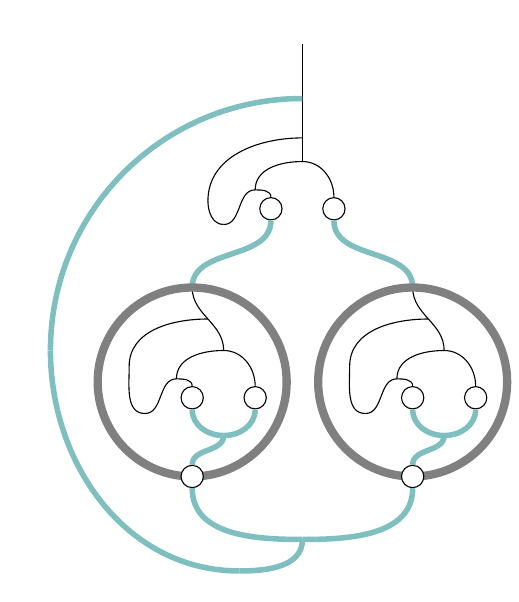
\begin{tikzpicture}[scale=0.4,auto,inner sep=1mm]
\coordinate (topr) at (0,2); % top of the bottom promoted 2
%\coordinate (comp) at (0,4) {};
\node (vtop) at ($ (topr) + (0,8) $) {};
\coordinate (meet) at ($ (vtop) - (0,2) $); % where the curved !( A -o A ) arc meets at the top

\draw (meet) to (vtop);

% ----------The Church 2 on top
\coordinate (2o) at ($ (topr) + (0,4) $);
\coordinate (2left_meet) at ($ (2o) - (1.5, 0.9) $);
\draw[out=90,in=180] (2left_meet) to (2o);

% Coproduct and derelictions
\dernode (2R) at ($ (2o) + (1,-1.5) $) {};
\dernode (2L) at ($ (2o) + (-1,-1.5) $) {};
\draw[out=90,in=0] (2R) to (2o);

% The A line curl from bottom to top
\coordinate (2left_curve) at ($ (2o) - (2.5, 2) $);
\coordinate (2left_curve_mid) at ($ (2o) - (3,1.25) $);
\coordinate (2first_meeting_top) at ($ (2o) + (0,0.75) $);
\draw[out=90,in=0] (2L) to (2left_meet);
\draw[out=0,in=180] (2left_curve) to (2left_meet);
\draw[out=180,in=270] (2left_curve) to (2left_curve_mid);
\draw[out=90,in=180] (2left_curve_mid) to (2first_meeting_top);
\draw (2o) to (meet);

%\draw[out=90,in=270] (2join_at_top) to (meet);
\drawbang[out=90,in=270] ($ (topr) + (-3.5,0) $) to (2L);
\drawbang[out=90,in=270] ($ (topr) + (3.5,0) $) to (2R);

% -------- promoted 2 LEFT ---------
% All coordinates are relative to the composition vertex (o), which itself
% has its coordinates derived from topr. This is the only link to the outside namespace.
\coordinate (o) at ($ (topr) + (-2.5,-2) $);
\coordinate (ellipse_center) at ($ (o) - (1,1) $);
\coordinate (elbow) at ($ (o) - (3, 0.5) $);
\coordinate (top_of_circle) at ($ (o) + (-1,2) $);
\draw[out=90,in=270] (o) to (top_of_circle);
\drawprom (ellipse_center) ellipse (3cm and 3cm); % outer boundary
\dernode (bottomr) at ($ (o) - (1,4) $) {};
\dernode (R) at ($ (o) + (1, -1.5) $) {}; % right dereliction
\dernode (L) at ($ (o) - (1,1.5) $) {}; % left dereliction
\coordinate (left_curve) at ($ (o) - (2.5,2) $);
\coordinate (left_meet) at ($ (o) - (1.5, 0.9) $);
\coordinate (delta) at ($ (o) - (0, 2.7) $); % coproduct vertex
\draw[out=90,in=0] (R) to node [swap] {} (o);
\drawbang[out=0,in=270] (delta) to (R);
\drawbang[out=180,in=270] (delta) to (L);
\drawbang[out=90,in=270] (bottomr) to (delta);
\draw[out=90,in=180] (left_meet) to (o);
\draw[out=90,in=0] (L) to (left_meet);
\draw[out=0,in=180] (left_curve) to (left_meet);
\draw[out=180,in=270] (left_curve) to (elbow);
\draw[out=90,in=180] (elbow) to ($ (o)!.5!(top_of_circle) $);
% ------ end promoted 2 ------

% -------- promoted 2 RIGHT ---------
% All coordinates are relative to the composition vertex (o), which itself
% has its coordinates derived from topr. This is the only link to the outside namespace.
\coordinate (o) at ($ (topr) + (4.5,-2) $);
\coordinate (ellipse_center) at ($ (o) - (1,1) $);
\coordinate (elbow) at ($ (o) - (3, 0.5) $);
\coordinate (top_of_circle) at ($ (o) + (-1,2) $);
\draw[out=90,in=270] (o) to (top_of_circle);
\drawprom (ellipse_center) ellipse (3cm and 3cm); % outer boundary
\dernode (right_bottomr) at ($ (o) - (1,4) $) {};
\dernode (R) at ($ (o) + (1, -1.5) $) {}; % right dereliction
\dernode (L) at ($ (o) - (1,1.5) $) {}; % left dereliction
\coordinate (left_curve) at ($ (o) - (2.5,2) $);
\coordinate (left_meet) at ($ (o) - (1.5, 0.9) $);
\coordinate (delta) at ($ (o) - (0, 2.7) $); % coproduct vertex
\draw[out=90,in=0] (R) to node [swap] {} (o);
\drawbang[out=0,in=270] (delta) to (R);
\drawbang[out=180,in=270] (delta) to (L);
\drawbang[out=90,in=270] (right_bottomr) to (delta);
\draw[out=90,in=180] (left_meet) to (o);
\draw[out=90,in=0] (L) to (left_meet);
\draw[out=0,in=180] (left_curve) to (left_meet);
\draw[out=180,in=270] (left_curve) to (elbow);
\draw[out=90,in=180] (elbow) to ($ (o)!.5!(top_of_circle) $);
% ------ end promoted 2 ------


% The loop from the bottom of the promoted 2 up to the top
\coordinate (curve) at (-8, 0);
\coordinate (very_bottom_turn) at (-2,-7);
\coordinate (very_bottom_delta) at (0,-6);
\drawbang[out=270,in=180] (curve) to (very_bottom_turn);
\drawbang[out=90,in=180] (curve) to (meet);
\drawbang[out=0,in=270] (very_bottom_turn) to (very_bottom_delta);
\drawbang[out=0,in=270] (very_bottom_delta) to (right_bottomr);
\drawbang[out=180,in=270] (very_bottom_delta) to (bottomr);
\end{tikzpicture}

&

\tagarray{\label{diagram_mult_2_2}}

\end{tabular}
\end{center}
At this point the promotions cancel with the derelictions by the identity \eqref{eq:prom_cancel_der}, ``releasing'' the pair of Church numerals contained in the promotion boxes. This yields the first equality below, while the second is an application of the general form of the identity represented by the transformation of diagrams in \eqref{eq:cutelim3} -- \eqref{eq:cutelim4}:
\begin{center}
\begin{tabular}{m{0.8cm} m{0.5cm} m{4.5cm} m{0.5cm} m{5cm}}
\eqref{diagram_mult_2_2} & = &
% ---------------------- TIKZ stacked 2's, RIGHT
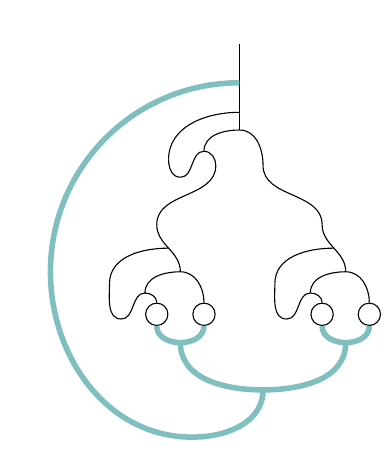
\begin{tikzpicture}[scale=0.3,auto,inner sep=1mm]
\coordinate (topr) at (0,2); % top of the bottom promoted 2
%\coordinate (comp) at (0,4) {};
\node (vtop) at ($ (topr) + (0,8) $) {};
\coordinate (meet) at ($ (vtop) - (0,2) $); % where the curved !( A -o A ) arc meets at the top

\draw (meet) to (vtop);

% ----------The Church 2 on top
\coordinate (2o) at ($ (topr) + (0,4) $);
\coordinate (2left_meet) at ($ (2o) - (1.5, 0.9) $);
\draw[out=90,in=180] (2left_meet) to (2o);

% Coproduct and derelictions
\coordinate (2R) at ($ (2o) + (1,-1.5) $);
\coordinate (2L) at ($ (2o) + (-1,-1.5) $);
\draw[out=90,in=0] (2R) to (2o);

% The A line curl from bottom to top
\coordinate (2left_curve) at ($ (2o) - (2.5, 2) $);
\coordinate (2left_curve_mid) at ($ (2o) - (3,1.25) $);
\coordinate (2first_meeting_top) at ($ (2o) + (0,0.75) $);
\draw[out=90,in=0] (2L) to (2left_meet);
\draw[out=0,in=180] (2left_curve) to (2left_meet);
\draw[out=180,in=270] (2left_curve) to (2left_curve_mid);
\draw[out=90,in=180] (2left_curve_mid) to (2first_meeting_top);
\draw (2o) to (meet);

%\draw[out=90,in=270] (2join_at_top) to (meet);
\draw[out=90,in=270] ($ (topr) + (-3.5,0) $) to (2L);
\draw[out=90,in=270] ($ (topr) + (3.5,0) $) to (2R);

% -------- promoted 2 LEFT ---------
% All coordinates are relative to the composition vertex (o), which itself
% has its coordinates derived from topr. This is the only link to the outside namespace.
\coordinate (o) at ($ (topr) + (-2.5,-2) $);
\coordinate (elbow) at ($ (o) - (3, 0.5) $);
\coordinate (top_of_circle) at ($ (o) + (-1,2) $);
\dernode (R) at ($ (o) + (1, -1.8) $) {}; % right dereliction
\dernode (L) at ($ (o) - (1,1.8) $) {}; % left dereliction
\coordinate (left_curve) at ($ (o) - (2.5,2) $);
\coordinate (left_meet) at ($ (o) - (1.5, 0.9) $);
\coordinate (delta) at ($ (o) - (0, 3) $); % coproduct vertex
\draw[out=90,in=0] (R) to node [swap] {} (o);
\drawbang[out=0,in=270] (delta) to (R);
\drawbang[out=180,in=270] (delta) to (L);
\draw[out=90,in=180] (left_meet) to (o);
\draw[out=90,in=0] (L) to (left_meet);
\draw[out=0,in=180] (left_curve) to (left_meet);
\draw[out=180,in=270] (left_curve) to (elbow);
\draw[out=90,in=270] (o) to (top_of_circle);
\draw[out=90,in=180] (elbow) to ($ (o)!.5!(top_of_circle) $);
% ------ end promoted 2 ------

% -------- promoted 2 RIGHT ---------
% All coordinates are relative to the composition vertex (o), which itself
% has its coordinates derived from topr. This is the only link to the outside namespace.
\coordinate (o) at ($ (topr) + (4.5,-2) $);
\coordinate (elbow) at ($ (o) - (3, 0.5) $);
\coordinate (top_of_circle) at ($ (o) + (-1,2) $);
\dernode (R) at ($ (o) + (1, -1.8) $) {}; % right dereliction
\dernode (L) at ($ (o) - (1,1.8) $) {}; % left dereliction
\coordinate (left_curve) at ($ (o) - (2.5,2) $);
\coordinate (left_meet) at ($ (o) - (1.5, 0.9) $);
\coordinate (right_delta) at ($ (o) - (0, 3) $); % coproduct vertex
\draw[out=90,in=0] (R) to node [swap] {} (o);
\drawbang[out=0,in=270] (right_delta) to (R);
\drawbang[out=180,in=270] (right_delta) to (L);
\draw[out=90,in=180] (left_meet) to (o);
\draw[out=90,in=0] (L) to (left_meet);
\draw[out=0,in=180] (left_curve) to (left_meet);
\draw[out=180,in=270] (left_curve) to (elbow);
\draw[out=90,in=270] (o) to (top_of_circle);
\draw[out=90,in=180] (elbow) to ($ (o)!.5!(top_of_circle) $);
% ------ end promoted 2 ------


% The loop from the bottom of the promoted 2 up to the top
\coordinate (curve) at (-8, 0);
\coordinate (very_bottom_turn) at (-2,-7);
\coordinate (very_bottom_delta) at (1,-5);
\drawbang[out=270,in=180] (curve) to (very_bottom_turn);
\drawbang[out=90,in=180] (curve) to (meet);
\drawbang[out=0,in=270] (very_bottom_turn) to (very_bottom_delta);
\drawbang[out=0,in=270] (very_bottom_delta) to (right_delta);
\drawbang[out=180,in=270] (very_bottom_delta) to (delta);
\end{tikzpicture}

& = &

% Final TikZ image for Church 4

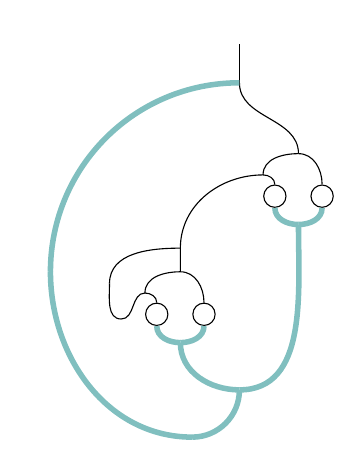
\begin{tikzpicture}[scale=0.3,auto,inner sep=1mm]
\coordinate (topr) at (0,2); % top of the bottom promoted 2
%\coordinate (comp) at (0,4) {};
\node (vtop) at ($ (topr) + (0,8) $) {};
\coordinate (meet) at ($ (vtop) - (0,2) $); % where the curved !( A -o A ) arc meets at the top

\draw (meet) to (vtop);

% -------- promoted 2 LEFT ---------
% All coordinates are relative to the composition vertex (o), which itself
% has its coordinates derived from topr. This is the only link to the outside namespace.
\coordinate (o) at ($ (topr) + (-2.5,-2) $);
\coordinate (elbow) at ($ (o) - (3, 0.5) $);
\coordinate (top_of_circle) at ($ (o) + (0,1) $);
\dernode (R) at ($ (o) + (1, -1.8) $) {}; % right dereliction
\dernode (L) at ($ (o) - (1,1.8) $) {}; % left dereliction
\coordinate (left_curve) at ($ (o) - (2.5,2) $);
\coordinate (left_meet) at ($ (o) - (1.5, 0.9) $);
\coordinate (delta) at ($ (o) - (0, 3) $); % coproduct vertex
\draw[out=90,in=0] (R) to node [swap] {} (o);
\drawbang[out=0,in=270] (delta) to (R);
\drawbang[out=180,in=270] (delta) to (L);
\draw[out=90,in=180] (left_meet) to (o);
\draw[out=90,in=0] (L) to (left_meet);
\draw[out=0,in=180] (left_curve) to (left_meet);
\draw[out=180,in=270] (left_curve) to (elbow);
\draw[out=90,in=270] (o) to (top_of_circle);
\draw[out=90,in=180] (elbow) to (top_of_circle);
% ------ end promoted 2 ------

% -------- promoted 2 RIGHT ---------
% All coordinates are relative to the composition vertex (o), which itself
% has its coordinates derived from topr. This is the only link to the outside namespace.
\coordinate (o) at ($ (topr) + (2.5,3) $);
\coordinate (elbow) at ($ (o) - (3, 0.5) $);
\coordinate (right_top_of_circle) at ($ (o) + (-1,2) $);
\dernode (R) at ($ (o) + (1, -1.8) $) {}; % right dereliction
\dernode (L) at ($ (o) - (1,1.8) $) {}; % left dereliction
\coordinate (left_curve) at ($ (o) - (2.5,2) $);
\coordinate (left_meet) at ($ (o) - (1.5, 0.9) $);
\coordinate (right_delta) at ($ (o) - (0, 3) $); % coproduct vertex
\draw[out=90,in=0] (R) to node [swap] {} (o);
\drawbang[out=0,in=270] (right_delta) to (R);
\drawbang[out=180,in=270] (right_delta) to (L);
\draw[out=90,in=180] (left_meet) to (o);
\draw[out=90,in=0] (L) to (left_meet);
% ------ end promoted 2 ------

\draw[out=90,in=180] (top_of_circle) to (left_meet);
\draw[out=90,in=270] (o) to (meet);

% The loop from the bottom of the promoted 2 up to the top
\coordinate (curve) at (-8, 0);
\coordinate (very_bottom_turn) at (-2,-7);
\coordinate (very_bottom_delta) at (0,-5);
\drawbang[out=270,in=180] (curve) to (very_bottom_turn);
\drawbang[out=90,in=180] (curve) to (meet);
\drawbang[out=0,in=270] (very_bottom_turn) to (very_bottom_delta);
\drawbang[out=0,in=270] (very_bottom_delta) to (right_delta);
\drawbang[out=180,in=270] (very_bottom_delta) to (delta);
\end{tikzpicture}
\end{tabular}
\end{center}
This last diagram is the denotation of $\church{4}$, so we conclude that (at least at the level of the denotations) the output of the program $\prf{\mathrm{mult}}_2$ on the input $\church{2}$ is $\church{4}$.

\vspace{1cm}

We examine the beginning of the cut-elimination process applied to the proof \eqref{cut_mult_2}. Our reference for cut-elimination is Melli\`{e}s \cite[\S 3.3]{mellies}. We encourage the reader to put the following series of proof trees side-by-side with the evolving diagrams in the above to see the correspondence between cut-elimination and diagram manipulation.

To begin, we expose the first layer of structure within $\prf{\mathrm{mult}}_2$ to obtain
\begin{center}
\AxiomC{$\church{2}$}
\noLine\UnaryInfC{$\vdots$}
\def\extraVskip{5pt}
\noLine\UnaryInfC{$\vdash \inta_A$}
\def\extraVskip{2pt}
\AxiomC{$\prf{\mathrm{mult}}_2'$}
\noLine\UnaryInfC{$\vdots$}
\def\extraVskip{5pt}
\noLine\UnaryInfC{$!(A \multimap A), \inta_A \vdash A \multimap A$}
\def\extraVskip{2pt}
\RightLabel{\scriptsize $\multimap R$}
\UnaryInfC{$\inta_A \vdash \inta_A$}
\RightLabel{\scriptsize cut}
\BinaryInfC{$\vdash \inta_A$}
\DisplayProof
\qquad
\tagarray{\label{cut_step_1}}
%\begin{tikzpicture}[scale=0.6,auto]
%\node (topr) at (1,4) {$\inta_A$};
%\bluenode (o) at (1,0) {};
%\bluenode (gam) at (2.5,-2) {};
%\draw[out=90,in=0] (gam) to node [swap]{$\inta_A$} (o);
%\drawbang[out=0,in=180] (-1.5,-2) to node {} (o);
%\drawbang[out=180,in=270] (-1.5,-2) to (-3,0);
%\drawbang[out=90,in=180] (-3,0) to (1,2);
%\draw (o) to node [swap] {$A \multimap A$} (1,2);
%\draw (1,2) to (topr);
%\end{tikzpicture}
%\end{tabular}
\end{center}
where $\prf{\mathrm{mult}}_2'$ indicates the ``remainder'' of the proof $\prf{\mathrm{mult}}_2$. For a cut against a proof whose last deduction rule is a right introduction rule for $\multimap$, the cut elimination procedure \cite[\S 3.11.10]{mellies} prescribes that \eqref{cut_step_1} be transformed to
\begin{center}
\AxiomC{$\church{2}$}
\noLine\UnaryInfC{$\vdots$}
\def\extraVskip{5pt}
\noLine\UnaryInfC{$\vdash \inta_A$}
\def\extraVskip{2pt}
\AxiomC{$\prf{\mathrm{mult}}_2'$}
\noLine\UnaryInfC{$\vdots$}
\def\extraVskip{5pt}
\noLine\UnaryInfC{$!(A \multimap A), \inta_A \vdash A \multimap A$}
\def\extraVskip{2pt}
\RightLabel{\scriptsize cut}
\BinaryInfC{$!(A \multimap A) \vdash A \multimap A$}
\RightLabel{\scriptsize $\multimap R$}
\UnaryInfC{$\vdash \inta_A$}
\DisplayProof
\qquad
\tagarray{\label{cut_step_2}}
\end{center}
If we fill in the content of $\prf{\mathrm{mult}}_2'$, this proof may be depicted as follows:
\begin{center}
\AxiomC{$\church{2}'$}
\noLine\UnaryInfC{$\vdots$}
\def\extraVskip{5pt}
\noLine\UnaryInfC{$!(A \multimap A)  \vdash A \multimap A$}
\def\extraVskip{2pt}
\UnaryInfC{$\vdash \inta_A$}
\AxiomC{$\church{2}'$}
\noLine\UnaryInfC{$\vdots$}
\def\extraVskip{5pt}
\noLine\UnaryInfC{$!(A \multimap A) \vdash A \multimap A$}
\def\extraVskip{2pt}
\RightLabel{\scriptsize prom}
\UnaryInfC{$!( A \multimap A) \vdash {!}(A \multimap A)$}
\AxiomC{}
\UnaryInfC{$A \multimap A \vdash A \multimap A$}
\RightLabel{\scriptsize$\multimap L$}
\BinaryInfC{$!(A \multimap A), \inta_A \vdash A \multimap A$}
\RightLabel{\scriptsize cut}
\BinaryInfC{$!(A \multimap A) \vdash A \multimap A$}
\RightLabel{\scriptsize $\multimap R$}
\UnaryInfC{$\vdash \inta_A$}
\DisplayProof
\qquad
\tagarray{\label{cut_step_3}}
\end{center}
The next cut-elimination step \cite[\S 3.8.2]{mellies} transforms this proof to
\begin{center}
\AxiomC{$\church{2}'$}
\noLine\UnaryInfC{$\vdots$}
\def\extraVskip{5pt}
\noLine\UnaryInfC{$!(A \multimap A) \vdash A \multimap A$}
\def\extraVskip{2pt}
\RightLabel{\scriptsize prom}
\UnaryInfC{$!( A \multimap A) \vdash {!}(A \multimap A)$}
\AxiomC{$\church{2}'$}
\noLine\UnaryInfC{$\vdots$}
\def\extraVskip{5pt}
\noLine\UnaryInfC{$!(A \multimap A) \vdash A \multimap A$}
\def\extraVskip{2pt}
\RightLabel{\scriptsize cut}
\BinaryInfC{$!(A \multimap A) \vdash A \multimap A$}
\AxiomC{}
\UnaryInfC{$A \multimap A \vdash A \multimap A$}
\RightLabel{\scriptsize cut}
\BinaryInfC{$!(A \multimap A) \vdash A \multimap A$}
\RightLabel{\scriptsize $\multimap R$}
\UnaryInfC{$\vdash \inta_A$}
\DisplayProof
\quad
\tagarray{\label{cut_step_4}}
\end{center}
As may be expected, cutting against an axiom rule does nothing, so this is equivalent to
\begin{prooftree}
\AxiomC{$\church{2}'$}
\noLine\UnaryInfC{$\vdots$}
\def\extraVskip{5pt}
\noLine\UnaryInfC{$!(A \multimap A) \vdash A \multimap A$}
\def\extraVskip{2pt}
\RightLabel{\scriptsize prom}
\UnaryInfC{$!( A \multimap A) \vdash {!}(A \multimap A)$}
\AxiomC{$\church{2}''$}
\noLine\UnaryInfC{$\vdots$}
\def\extraVskip{5pt}
\noLine\UnaryInfC{$!(A \multimap A), !(A \multimap A) \vdash A \multimap A$}
\def\extraVskip{2pt}
\RightLabel{\scriptsize ctr}
\UnaryInfC{$!(A \multimap A) \vdash A \multimap A$}
\RightLabel{\scriptsize cut}
\BinaryInfC{$!(A \multimap A) \vdash A \multimap A$}
\RightLabel{\scriptsize $\multimap R$}
\UnaryInfC{$\vdash \inta_A$}
\end{prooftree}
where $\church{2}''$ is a sub-proof of $\church{2}$. Here is the important step: cut-elimination replaces a cut of a promotion against a contraction by a pair of promotions \cite[\S 3.9.3]{mellies}. This step corresponds to the doubling of the promotion box in \eqref{diagram_mult_2_2}
\begin{prooftree}
\AxiomC{$\church{2}'$}
\noLine\UnaryInfC{$\vdots$}
\def\extraVskip{5pt}
\noLine\UnaryInfC{$!(A \multimap A) \vdash A \multimap A$}
\def\extraVskip{2pt}
\UnaryInfC{$!( A \multimap A) \vdash {!}(A \multimap A)$}
\AxiomC{$\church{2}'$}
\noLine\UnaryInfC{$\vdots$}
\def\extraVskip{5pt}
\noLine\UnaryInfC{$!(A \multimap A) \vdash A \multimap A$}
\def\extraVskip{2pt}
\UnaryInfC{$!( A \multimap A) \vdash {!}(A \multimap A)$}
\AxiomC{$\church{2}''$}
\noLine\UnaryInfC{$\vdots$}
\def\extraVskip{5pt}
\noLine\UnaryInfC{$!(A \multimap A), !(A \multimap A) \vdash A \multimap A$}
\def\extraVskip{2pt}
\RightLabel{\scriptsize cut}
\BinaryInfC{$!(A \multimap A), !(A \multimap A) \vdash A \multimap A$}
\RightLabel{\scriptsize cut}
\BinaryInfC{$!(A \multimap A), !(A \multimap A) \vdash A \multimap A$}
\RightLabel{\scriptsize ctr}
\UnaryInfC{$!(A \multimap A) \vdash A \multimap A$}
\RightLabel{\scriptsize $\multimap R$}
\UnaryInfC{$\vdash \inta_A$}
\end{prooftree}
We only sketch the rest of the cut-elimination process: next, the derelictions in $\church{2}''$ will be annihilate with the promotions in the two copies of $\church{2}'$ according to \cite[\S 3.9.1]{mellies}. Then there are numerous eliminations involving the right and left $\multimap$ introduction rules. %, which are not very interesting. %The point is that after the next step, cuts on formulas $!(A \multimap A)$ will be replaced by cuts on formulas $A \multimap A$, which are of lower complexity. 

\section{The geometry of interaction}\label{section:goi}

One interesting aspect of linear logic is Girard's program to study the semantics of the cut-elimination process; see \cite[\S III]{girard_towards} and \cite{girard_goi1,girard_goi2,girard_goi3}. The purpose of this section is to very briefly explain his idea. As mentioned in the Introduction, the three most common views on what the dynamical process of computation ``is'' are the execution of a Turing machine, $\beta$-reduction in the $\lambda$-calculus, and cut-elimination in sequent calculus. At a first approach we notice that common to all three of these models of computation is a tension between the \emph{implicit} and the \emph{explicit}. We use the computation of Section \ref{section:cut_elim} to explain. 

Consider the proofs $\prf{\mathrm{mult}}_2$ and $\church{2}$ and their cut $\prf{\mathrm{mult}}_2 \l \church{2}$. The latter is equivalent under cut-elimination to the cut-free proof $\church{4}$. Since this answer is derived from a deterministic algorithm -- cut-elimination -- the knowledge is certainly \emph{implicit} in the proof $\prf{\mathrm{mult}}_2 \l \church{2}$. But some work was necessary to convert this implicit truth into \emph{explicit} truth. Although this example is a trivial one, the reader can easily imagine a similar calculation whose answer is not as apparent as $2 \times 2 = 4$ -- or, put aside arithmetic and note that the answer $\church{4}$ is not obvious from a glance at the diagram \eqref{cut_mult_2}. This \emph{explicitation} is a fundamental aspect of computation, but as the reader can already appreciate, it is difficult to define precisely what we mean by ``explicitness''. This is the problem that a mathematical model of cut-elimination is designed to solve.
% Moreover, this implicitness arises from the act of identifying the structured object $\inta_A$ which is the output of $\church{2}$ with the ``same'' structured object $\inta_A$ which is the input of $\prf{\mathrm{mult}}_2$.\footnote{The algebraically minded reader who is amused by the scare quotes on the word ``same'' might like to reflect on the distinction between an underived and a derived tensor product with the diagonal bimodule.}
\\

However, this explicitation process is missing from most mathematical models of computation, which assign to the syntactical gadgets of Turing machines, $\lambda$-calculus or logic mathematical objects and transformations between them. To elaborate: suppose that in linear logic that we have proofs $\pi$ of $A \vdash B$ and $\rho$ of $B \vdash C$, and let $\rho \l \pi$ denote the cut of one against the other, as displayed in the following proof tree:
\begin{center}
\AxiomC{$\pi$}
\noLine\UnaryInfC{$\vdots$}
\def\extraVskip{5pt}
\noLine\UnaryInfC{$A \vdash B$}
\def\extraVskip{2pt}
\AxiomC{$\rho$}
\noLine\UnaryInfC{$\vdots$}
\def\extraVskip{5pt}
\noLine\UnaryInfC{$B \vdash C$}
\def\extraVskip{2pt}
\RightLabel{\scriptsize cut}
\BinaryInfC{$A \vdash C$}
\DisplayProof
\qquad
\tagarray{\label{goi_prooftree}}
\end{center}
Let $\widetilde{\rho\l\pi}$ denote the cut-free proof of $A \vdash C$ produced from $\rho \l \pi$ by the cut-elimination process. We regard this as the output of the program $\rho$ computed on the input $\pi$. In the vector space semantics there is a commutative diagram of linear maps
\[
\xymatrix@C+2pc{
& \den{B} \ar[dr]^-{\den{\rho}}\\
\den{A} \ar[ur]^-{\den{\pi}}\ar[rr]_-{\den{\rho\l\pi} = \den{\widetilde{\rho\l\pi}}} & & \den{C}
}
\]
On this level, the calculation of output from input is a one-step affair $\den{\pi} \mapsto \den{\rho} \circ \den{\pi}$. This may be contrasted with the syntax, where two steps are involved
\begin{equation}\label{eq:cut_elim_step}
\pi \longmapsto \rho \l \pi \longmapsto \widetilde{\rho \l \pi}\,.
\end{equation}
The point is that this second step, cut-elimination, is completely invisible in the semantics since both $\rho \l \pi$ and its normalisation have the same denotation -- by construction. The explicitation that happens in the syntax is absent in the semantics.

Girard proposed \cite{girard_towards} that we should look instead for semantics in which the denotations of $\rho \l \pi$ and $\widetilde{\rho\l\pi}$ are distinct and there are ``dynamics'' which generate the latter from the former. He refers to the field of study of such dynamics as the \emph{geometry of interaction}.\footnote{The categorically minded reader will detect the hint of higher-categories: it would be natural to expect that the denotations of a proof and its cut-free normalisation should be $1$-morphisms connected by some structure on the level of $2$-morphisms which models cut-elimination.} The first example of such a semantics constructed by Girard in \cite{girard_goi1} has been influential, although arguably it is still a bit mysterious. Since the $\lambda$-calculus may be translated into intuitionistic logic, and from there into intuitionistic linear logic, any semantics of linear logic yields a method for the execution of programs in the $\lambda$-calculus. One practical application of Girard's geometry of interaction model of linear logic is that it yields a method of executing programs in which the elementary reduction steps are local -- that is, they do not dependent on global coordination \cite{danos_regnier1,danos_regnier2}. This is closely related to famous work of Lamping on optimal reduction in the $\lambda$-calculus \cite{Gonthier}.

\appendix

\section{Tangents and proofs}\label{section:example_lifting}

%In this appendix we consider various examples of the lifting formula in Theorem \ref{theorem:describe_lifting}, centered around the notion of tangent vectors at proof denotations. 


%\begin{definition}\label{defn:nonlinear_deno} Given a proof $\pi$ of a sequent $!A \vdash B$ let $\langle \pi \rangle$ denote the function
%\begin{gather*}
%\langle \pi \rangle: \den{A} \lto \den{B},\\
%\langle \pi \rangle(P) = \den{\pi} \ket{o}_P\,.
%\end{gather*}
%\end{definition}

%One interesting example of lifting involves tangent vectors at proofs.

\begin{example}\label{example:tangent_coalgebra} Let $\cat{T}$ denote the dual of the finite-dimensional algebra $k[t]/(t^2)$. It has a $k$-basis $1 = 1^*$ and $\varepsilon = t^*$ and coproduct $\Delta$ and counit $u$ defined by
\[
\Delta(1) = 1 \otimes 1, \quad \Delta( \varepsilon ) = 1 \otimes \varepsilon + \varepsilon \otimes 1, \quad u(1) = 1, \quad u(\varepsilon) = 0\,.
\]
Recall that a tangent vector at a point $x$ on a scheme $X$ is a morphism $\Spec(k[t]/t^2) \lto X$ sending the closed point to $x$. Given a finite-dimensional vector space $V$ and $R = \Sym(V^*)$ with $X = \Spec(R)$, this is equivalent to a morphism of $k$-algebras
\[
\varphi: \Sym(V^*) \lto k[t]/t^2
\]
with $\varphi^{-1}( (t) ) = x$. Such a morphism of algebras is determined by its restriction to $V^*$, which as a linear map $\varphi|_{V^*}: V^* \lto k[t]/t^2$ corresponds to a pair of elements $(P, Q)$ of $V$, where $\varphi( \tau ) = \tau(P) \cdot 1 + \tau(Q) \cdot t$. Then $\varphi$ sends a polynomial $f$ to
\[
\varphi(f) = f(P) \cdot 1 + \partial_Q( f )|_P \cdot t\,.
\]
The map $\varphi|_{V^*}$ is also determined by its dual, which is a linear map $\phi: \cat{T} \lto V$. By the universal property, this lifts to a morphism of coalgebras $\Phi: \cat{T} \lto {!}V$. If $\phi$ is determined by a pair of points $(P,Q) \in V^{\oplus 2}$ as above, then it may checked directly that
\[
\Phi( 1 ) = \ket{o}_P, \qquad \Phi( \varepsilon ) = \ket{ Q }_P
\]
is a morphism of coalgebras lifting $\phi$.
%Using the dual of $k[t]/t^N$ for various powers $N$ we may in this way make an identification between ${!} V$ and the infinite jet-space of $V$.
\end{example}

Motivated by this example, we make a preliminary investigation into tangent vectors at proof denotations. Let $A,B$ be types with finite-dimensional denotations $\den{A}, \den{B}$.

\begin{definition} Given a proof $\pi$ of $\vdash A$ a \emph{tangent vector} at $\pi$ is a morphism of coalgebras $\theta: \cat{T} \lto {!} \den{A}$ with the property that $\theta(1) = \ket{o}_{\den{\pi}}$, or equivalently that the diagram
\begin{equation}
\xymatrix@C+2pc{
k \ar[d]_-{1} \ar[r]^-{\den{\pi}} & \den{A}\\
\cat{T} \ar[r]_-{\theta} & {!} \den{A} \ar[u]_-{d}
}
\end{equation}
commutes. The space of tangent vectors at $\pi$ is denoted $T_{\pi}$.
\end{definition}

It follows from Example \ref{example:tangent_coalgebra} that there is a linear isomorphism
\[
\den{A} \lto T_{\pi}
\]
sending $Q \in \den{A}$ to the coalgebra morphism $\theta$ with $\theta(1) = \ket{o}_{\den{\pi}}$ and $\theta(\varepsilon) = \ket{Q}_{\den{\pi}}$. 

Note that the denotation of a program not only maps inputs to outputs (if we identify inputs and outputs with vacuum vectors) but also tangent vectors to tangent vectors. To wit, if $\rho$ is a proof of a sequent $!A \vdash B$ with denotation $\lambda: {!} \den{A} \lto \den{B}$, then composing a tangent vector $\theta$ at a proof $\pi$ of $\vdash A$ with the lifting $\Lambda$ of $\lambda$ leads to a tangent vector at the cut of $\rho$ against the promotion of $\pi$. That is, the linear map
\begin{equation}\label{eq:fake_tangent_map}
\xymatrix@C+2pc{
\cat{T} \ar[r]^-{\theta} & ! \den{A} \ar[r]^-{\Lambda} & ! \den{B}
}
\end{equation}
is a tangent vector at the following proof, which we denote $\rho \l \pi$
\begin{prooftree}
\AxiomC{$\pi$}
\noLine\UnaryInfC{$\vdots$}
\def\extraVskip{5pt}
\noLine\UnaryInfC{$\vdash A$}
\def\extraVskip{2pt}
\RightLabel{\scriptsize prom}
\UnaryInfC{$\vdash {!} A$}
\AxiomC{$\rho$}
\noLine\UnaryInfC{$\vdots$}
\def\extraVskip{5pt}
\noLine\UnaryInfC{$!A \vdash B$}
\def\extraVskip{2pt}
\RightLabel{\scriptsize cut}
\BinaryInfC{$\vdash B$}
\end{prooftree}
By Theorem \ref{theorem:describe_lifting} the linear map of tangent spaces induced in this way by $\rho$ is
\begin{gather}
\den{A} \cong T_{\pi} \lto T_{\rho\l\pi} \cong \den{B}\label{eq:tangent_map_logic}\\
Q \longmapsto \lambda \ket{Q}_{\den{\pi}}\nonumber
\end{gather}

When $\rho$ computes a smooth map of differentiable manifolds, this map can be compared with an actual map of tangent spaces. We examine $\rho = \church{2}$ below. It would be interesting to understand these maps in more complicated examples; this seems to be related to the differential $\lambda$-calculus \cite{ehrhard_difflambda,ehrhard_difflambda2}, but we have not tried to work out the precise connection.

\begin{example}\label{example:tangent_to_2} When $k = \mathbb{C}$ and $Z = \den{\church{2}}_{nl}$ we have by Lemma \ref{lemma:nonlinear_recover}
\[
Z: M_n(\mathbb{C}) \lto M_n(\mathbb{C}), \qquad Z(\alpha) = \alpha^2\,.
\]
The tangent map of the smooth map of manifolds $Z$ at $\alpha$ is $(Z_*)_\alpha( \nu ) = \{ \nu, \alpha \}$. When $\alpha$ is the denotation of some proof $\pi$ of $\vdash A \multimap A$ this agrees with the tangent map assigned in \eqref{eq:tangent_map_logic} to the proof $\church{2}$ at $\pi$, using \eqref{eq:church_2_den}.
\end{example}

\bibliographystyle{amsalpha}
\providecommand{\bysame}{\leavevmode\hbox to3em{\hrulefill}\thinspace}
\providecommand{\href}[2]{#2}
\begin{thebibliography}{BHLS03}

\bibitem{abramsky}
S.~Abramsky, \textsl{Computational interpretations of linear logic}, Theoretical Computer Science, 1993.

\bibitem{abramsky4}
S.~Abramsky, \textsl{Retracting some paths in process algebra}, In CONCUR 96, Springer Lecture Notes in Computer Science \textbf{1119}, 1--17, 1996.

\bibitem{abramsky2}
S.~Abramsky, \textsl{Geometry of {I}nteraction and linear combinatory algebras}, Mathematical Structures in Computer Science, \textbf{12}, 625--665, 2002.

\bibitem{abramsky3}
S.~Abramsky and R.~Jagadeesan, \textsl{New foundations for the {G}eometry of {I}nteraction}, Information and Computation \textbf{111} (1), 53--119, 1994.

\bibitem{anel}
M.~Anel, A.~Joyal, \textsl{Sweedler theory of (co)algebras and the bar-cobar constructions}, \href{http://arxiv.org/abs/1309.6952}{[arXiv:1309.6952]}

\bibitem{atiyah}
M.~Atiyah, \textsl{Topological quantum field theories}, Publications Math\'{e}matique de l'IH\'{E}S 68, 175--186, 1989.

\bibitem{baez}
J.~Baez and M.~Stay, \textsl{Physics, topology, logic and computation: a Rosetta stone}, in B. Coecke (ed.) New Structures for Physics, Lecture Notes in Physics 813, Springer, Berlin, 95--174, 2011

\bibitem{barr}
M.~Barr, \textsl{Coalgebras over a commutative ring}, Journal of Algebra 32, 600--610, 1974.

\bibitem{barr_auto}
\bysame, \textsl{$\star$-autonomous categories}, Number 752 in Lecture Notes in Mathematics. Springer-Verlag, 1979.

\bibitem{barr_acc}
\bysame, \textsl{Accessible categories and models of linear logic}, Journal of Pure and Applied Algebra, 69(3):219--232, 1990.

\bibitem{barr_autolin}
\bysame, {$?$-autonomous categories and linear logic}, Mathematical Structures in Computer Science, 1(2):159--178, 1991.

\bibitem{barr_chu}
\bysame, \textsl{The {C}hu construction: history of an idea}, Theory and Applications of Categories, Vol. 17, No. 1, 10--16, 2006.

\bibitem{benton}
N.~Benton, \textsl{A mixed linear and non-linear logic; proofs, terms and models}, in Proceedings of Computer Science Logic 94, vol. 933 of Lecture Notes in Computer Science, Verlag, 1995.

\bibitem{benton_etal}
N.~Benton, G.~Bierman, V.~de Paiva and M.~Hyland, \textsl{Term assignment for intuitionistic linear logic}, Technical report 262, Computer Laboratory, University of Cambridge, 1992.

\bibitem{block-leroux} 
R.~Block, P.~Leroux, \textsl{Generalized dual coalgebras of algebras, with applications to cofree coalgebras}, J. Pure Appl. Algebra 36, no. 1, 15--21, 1985.

\bibitem{blute}
R.~Blute, \textsl{Hopf algebras and linear logic}, Mathematical Structures in Computer Science, 6(2):189--217, 1996.

\bibitem{blute_scott}
R.~Blute and P.~Scott, \textsl{Linear {L}a\"{u}chli semantics}, Annals of Pure and Applied Logic, 77:101--142, 1996.

\bibitem{blue_book}
\bysame, \textsl{Category theory for linear logicians}, Linear Logic in Computer Science 316: 3--65, 2004.

\bibitem{blute_fock}
R.~Blute, P.~Panangaden, R.~Seely, \textsl{Fock space: a model of linear exponential types}, in: Proc. Ninth Conf. on Mathematical Foundations of Programming Semantics, Lecture Notes in Computer Science, Vol. 802, Springer, Berlin, 1--25, 1994.

\bibitem{bott}
R.~Bott and L.W.~Tu, \textsl{Differential forms in {A}lgebraic {T}opology}, Graduate Texts in Mathematics, \textbf{82}, Springer, 1982.

\bibitem{ct1007.2679}
A.~{C\u ald\u araru} and S.~Willerton, \textsl{The Mukai pairing, I: a categorical approach},
New York Journal of Mathematics \textbf{16}, 61--98, 2010
  \href{http://arxiv.org/abs/0707.2052}{[arXiv:0707.2052]}.
  
\bibitem{lgdual}
N.~Carqueville and D.~Murfet, \textsl{Adjunctions and defects in {L}andau-{G}inzburg models}, \href{http://arxiv.org/abs/1208.1481}{[arXiv:1208.1481]}.

\bibitem{cr0909.4381}
N.~Carqueville and I.~Runkel, \textsl{On the monoidal structure of matrix bi-factorisations}, J. Phys.
  A: Math. Theor. \textbf{43} 275--401, 2010
  \href{http://arxiv.org/abs/0909.4381}{[arXiv:0909.4381]}.

\bibitem{church}
A.~Church, \textsl{The {C}alculi of {L}ambda-conversion}, Princeton University Press, Princeton, N. J. 1941.

\bibitem{danos}
V.~Danos and J.-B.~Joinet, \textsl{Linear logic and elementary time}, Information and Computation 183, 123--127, 2003.

\bibitem{danos_regnier1}
V.~Danos and L.~Regnier, \textsl{Local and {A}synchronous beta-reduction (an analysis of {G}irard's execution formula)} in: Springer Lecture Notes in Computer Science \textbf{8}, 296--306, 1993.

\bibitem{danos_regnier2}
V.~Danos and L.~Regnier, \textsl{Proof-nets and the Hilbert space}, in (Girard \textsl{et. al.} 1995), 307--328, 1995.

\bibitem{denning}
P.~J.~Denning, \textsl{Ubiquity symposium ``What is computation?''}: opening statement, Ubiquity 2010. Available on the \href{http://ubiquity.acm.org/article.cfm?id=1870596}{Ubiquity website}.

\bibitem{dm1102.2957}
T.~Dyckerhoff and D.~Murfet, \textsl{Pushing forward matrix factorisations}, Duke Math. J. Volume 162, Number 7 1249--1311, 2013 \href{http://arxiv.org/abs/1102.2957}{[arXiv:1102.2957]}.

\bibitem{ehrhard}
T.~Ehrhard, \textsl{Finiteness spaces}, Math. Structures Comput. Sci. 15 (4) 615--646, 2005.

\bibitem{ehrhard_kothe}
\bysame, \textsl{On {K}\"othe sequence spaces and linear logic}, Mathematical Structures in Computer Science 12.05, 579--623, 2002.

\bibitem{ehrhard_difflambda}
T.~Ehrhard and L.~Regnier, \textsl{The differential lambda-calculus}, Theoretical Computer Science 309.1: 1--41, 2003.

\bibitem{ehrhard_difflambda2}
\bysame, \textsl{Differential interaction nets}, Theoretical Computer Science 364.2: 166--195, 2006.

\bibitem{gentzen}
G.~Gentzen, \textsl{The Collected Papers of Gerhard Gentzen}, (Ed. M. E. Szabo), Amsterdam, Netherlands: North-Holland, 1969.

\bibitem{getzler}
E.~Getzler, P.~Goerss, \emph{A model category structure for differential graded coalgebras}, preprint, 1999.
  
\bibitem{girard_llogic}
J.-Y.~Girard, \textsl{Linear Logic}, Theoretical Computer Science 50 (1), 1--102, 1987.

\bibitem{girard_normal}
\bysame, \textsl{Normal functors, power series and the $\lambda$-calculus} Annals of Pure and Applied
Logic, 37: 129--177, 1988.

\bibitem{girard_goi1}
\bysame, \textsl{Geometry of {I}nteraction I: {I}interpretation of {S}ystem {F}}, in Logic Colloquium '88, ed. R.~Ferro, et al. North-Holland, 221--260, 1988.

\bibitem{girard_goi2}
\bysame, \textsl{Geometry of {I}nteraction II: {D}eadlock-free {A}lgorithms}, COLOG-88, Springer Lecture Notes in Computer Science \textbf{417}, 76--93, 1988.

\bibitem{girard_goi3}
\bysame, \textsl{Geometry of {I}nteraction III: {A}ccommodating the {A}dditives}, in (Girard \textsl{et al}. 1995), pp.1--42.

\bibitem{girard_towards}
\bysame, \textsl{Towards a geometry of interaction}, In J.~W.~Gray and A.~Scedrov, editors, Categories in Computer Science and Logic, volume 92 of Contemporary Mathematics, 69--108, AMS, 1989.

\bibitem{girard_complexity}
\bysame, \textsl{Light linear logic}, Information and Computation 14, 1995.

\bibitem{girard_coherentbanach}
\bysame, \textsl{Coherent {B}anach spaces: a continuous denotational semantics}, Theoretical Computer Science, 227: 275--297, 1999.

\bibitem{girard_prooftypes}
J.-Y.~Girard, Y.~Lafont, and P.~Taylor, \textsl{Proofs and Types}, Cambridge Tracts in Theoretical Computer Science 7 ,Cambridge University Press, 1989.

\bibitem{Gonthier}
G.~Gontheir, M.~Abadi and J.-J.~L\'{e}vy, \textsl{The geometry of optimal lambda reduction}, in 9th Annual IEEE Symp. on Logic in Computer Science (LICS), 15--26, 1992.
  
\bibitem{haghverdi}
E.~Haghverdi and P.~Scott, \textsl{Geometry of {I}nteraction and the dynamics of prood reduction: a tutorial}, in New Structures for Physics, Lecture notes in Physics \textbf{813}, 357--417, 2011.
  
\bibitem{hazewinkel}
H.~Hazewinkel, \textsl{Cofree coalgebras and multivariable recursiveness}, J. Pure Appl. Algebra 183, no. 1--3, 61--103, 2003.

\bibitem{hyland}
M.~Hyland and A.~Schalk, \textsl{Glueing and orthogonality for models of linear logic}, Theoretical Computer Science, 294: 183--231, 2003.

\bibitem{JSGoTCI}
A.~Joyal and R.~Street, \textsl{The geometry of tensor calculus I}, Advances in Math. \textbf{88}, 55--112, 1991.

\bibitem{JSGoTCII}
A.~Joyal and R.~Street, \textsl{The geometry of tensor calculus II}, 
draft available at 
\href{http://maths.mq.edu.au/~street/GTCII.pdf}{http://maths.mq.edu.au/\textasciitilde street/GTCII.pdf}

\bibitem{joyal_trace}
A.~Joyal, R.~Street and D.~Verity, \textsl{Traced monoidal categories}, Math. Proc. Camb. Phil. Soc. 119, 447--468, 1996.

\bibitem{khovdia}
M.~Khovanov, \textsl{Categorifications from planar diagrammatics}, Japanese J. of Mathematics \textbf{5}, 153--181, 2010 \href{http://arxiv.org/abs/1008.5084}{[arXiv:1008.5084]}.
  
\bibitem{lafont}
Y.~Lafont, \textsl{The {L}inear {A}bstract {M}achine}, Theoretical Computer Science, 59 (1,2):157--180, 1988.

\bibitem{lambek}
J.~Lambek and P.~J.~Scott, \textsl{Introduction to higher order categorical logic}, Cambridge Studies in Advanced Mathematics, vol. 7, Cambridge University Press, Cambridge, 1986.

\bibitem{ladia}
A.~D.~Lauda, \textsl{An introduction to diagrammatic algebra and categorified quantum $\mathfrak{sl}_2$}, Bulletin of the Institute of Mathematics Academia Sinica (New Series), Vol. \textbf{7}, No. 2, 165--270, 2012 \href{http://arxiv.org/abs/1106.2128}{[arXiv:1106.2128]}.

\bibitem{mccarthy}
J.~McCarthy, \textsl{Recursive functions of symbolic expressions and their computation by machine, Part I.}, Communications of the ACM 3.4: 184--195, 1960.

\bibitem{McNameethesis}
D.~McNamee, \textsl{On the mathematical structure of topological defects in
  {L}andau-{G}inzburg models}, MSc Thesis, Trinity College Dublin, 2009.
  
\bibitem{mellies_dia}
P.-A.~Melli\`{e}s, \textsl{Functorial boxes in string diagrams}, In Z. \'{E}sik, editor, Computer Science Logic,
volume 4207 of Lecture Notes in Computer Science, pages 1--30, Springer Berlin / Heidelberg,
2006.

\bibitem{mellies}
P-A.~Melli\`{e}s, \textsl{Categorical semantics of linear logic}, in : Interactive models of computation and program behaviour, Panoramas et Synth\`{e}ses $27$, Soci\'{e}t\'{e} Math\'{e}matique de France, 2009.

\bibitem{mellies2}
P.-A.~Melli\`{e}s, N.~Tabareau, C.~Tasson, \textsl{An explicit formula for the free exponential modality of linear logic}, in: 36th International Colloquium on Automata, Languages and Programming, July 2009, Rhodes, Greece, 2009.

\bibitem{murfet}
D.~Murfet, \textsl{Computing with cut systems}, \href{http://arxiv.org/abs/1402.4541}{[arXiv:1402.4541]}.

\bibitem{murfet_coalg}
D.~Murfet, \textsl{On Sweedler's cofree cocommutative coalgebra}, \href{http://arxiv.org/abs/1406.5749}{[arXiv:1406.5749]}.

\bibitem{pagani}
M.~ Pagani and L.~Tortora de Falco.\textsl{Strong normalization property for second order linear logic}, Theoretical Computer Science 411.2 (2010): 410--444.

\bibitem{pv}
A.~Polishchuk and A.~Vaintrob, \textsl{Chern characters and {H}irzebruch-{R}iemann-{R}och formula for matrix factorizations}, Duke Mathematical Journal 161.10: 1863--1926, 2012 \href{http://arxiv.org/abs/1002.2116}{[arXiv:1002.2116]}. 

\bibitem{schreiber}
U.~Schreiber, \textsl{Quantization via {L}inear homotopy types}, \href{http://arxiv.org/abs/1402.7041}{[arXiv:1402.7041]}.

\bibitem{scott}
D.~Scott, \textsl{Data types as lattices}, SIAM Journal of computing, 5:522--587, 1976.

\bibitem{scott_talk}
\bysame, \textsl{The {L}ambda calculus, then and now}, available on \href{http://www.youtube.com/watch?v=7cPtCpyBPNI}{YouTube} with \href{http://turing100.acm.org/lambda_calculus_timeline.pdf}{lecture notes}, 2012.

\bibitem{seely}
R.~Seely, \textsl{Linear logic, star-autonomous categories and cofree coalgebras}, Applications of categories in logic and computer science, Contemporary Mathematics, 92, 1989.

\bibitem{selinger}
P.~Selinger, \textsl{Lecture notes on the {L}ambda calculus}, \href{http://arxiv.org/abs/0804.3434}{[arXiv:0804.3434]}.

\bibitem{shirahata}
M.~Shirahata, \textsl{Geometry of {I}nteraction explained}, available \href{http://www.kurims.kyoto-u.ac.jp/~hassei/algi-13/kokyuroku/19_shirahata.pdf}{online}.

\bibitem{soare}
R.~I.~Soare, \textsl{Computability and {I}ncomputability}, in CiE 2007: Computation and Logic in the Real World, LNCS 4497, Springer, 705--715.
  
\bibitem{sweedler}
M.~Sweedler, \textsl{Hopf Algebras}, W.~A.~Benjamin, New York, 1969.

\bibitem{valiron}
B.~Valiron and S.~Zdancewic, \textsl{Finite vector spaces as model of simply-typed lambda-calculi}, \href{http://arxiv.org/abs/1406.1310v1}{[arXiv:1406.1310]}.

\bibitem{quillen}
D.~Quillen, \textsl{Rational homotopy theory}, The Annals of Mathematics, Second Series, Vol. 90, No. 2, 205--295, 1969.

\bibitem{univalent}
The Univalent Foundations Program, \textsl{Homotopy {T}ype {T}heory: {U}nivalent {F}oundations of {M}athematics}, Institute for Advanced Study (Princeton), 2013.

\bibitem{Yoshino90}
Y.~Yoshino, \emph{Cohen-{M}acaulay modules over {C}ohen-{M}acaulay rings},
  London Mathematical Society Lecture Note Series, vol. 146, Cambridge
  University Press, Cambridge, 1990. 
  
\bibitem{witten}
E.~Witten, \textsl{Topological quantum field theory}, \textsl{Communications in Mathematical Physics}, 117 (3), 353--386, 1988.

\end{thebibliography}

\end{document}

\section{Cuts}

\begin{example} For any type $A$, addition of two $A$-integers is represented by the following cut-free proof $\prf{\mathrm{add}}$ of $\inta_A, \inta_A \vdash \inta_A$
%\scalebox{0.6}{
%\parbox{2cm}{
\begin{prooftree}
\AxiomC{}
\UnaryInfC{$!(A \multimap A) \vdash {!}(A \multimap A)$}
\AxiomC{}
\UnaryInfC{$!(A \multimap A) \vdash {!}(A \multimap A)$}
\AxiomC{}
\UnaryInfC{$A \vdash A$}
\AxiomC{}
\UnaryInfC{$A \vdash A$}
\AxiomC{}
\UnaryInfC{$A \vdash A$}
\RightLabel{\scriptsize$\multimap L$}
\BinaryInfC{$A, A \multimap A \vdash A$}
\RightLabel{\scriptsize$\multimap L$}
\BinaryInfC{$A, A \multimap A, A \multimap A \vdash A$}
\RightLabel{\scriptsize$\multimap R$}
\UnaryInfC{$A \multimap A, A \multimap A \vdash A \multimap A$}
\RightLabel{\scriptsize$\multimap L$}
\BinaryInfC{$!(A \multimap A), \inta_A, A \multimap A \vdash A \multimap A$}
\RightLabel{\scriptsize$\multimap L$}
\BinaryInfC{$!(A \multimap A), \inta_A, \inta_A \vdash A \multimap A$}
\RightLabel{\scriptsize$\multimap R$}
\UnaryInfC{$\inta_A, \inta_A \vdash \inta_A$}
\end{prooftree}
The denotation of which is a morphism
\[
\den{\prf{\mathrm{add}}}: \den{\inta_A} \otimes \den{\inta_A} \lto \den{\inta_A}
\]
To actually perform an addition, we would \emph{cut} two Church numerals against this proof, for instance with the following proof tree:
\[
blah
\]
The denotation of this combined proof is the composite
\[
\den{\prf{\mathrm{add}}} \circ ( \den{\church{m}} \otimes \den{\church{n}} ): k \lto \den{\inta_A}\,.
\]
The cut-elimination process gives us a deterministic algorithm for replacing this proof by a cut-free proof of the same formula $\inta_A$. It is a worthwhile exercise to perform this cut-elimination and verify that the resulting cut-free proof is precisely the integer $\church{n+m}$. Alternatively one can prove that the Church numerals are the \emph{only} cut-free proofs of $\inta_A$ and then use the semantics to distinguish between them.
\end{example}
